\documentclass[aps,prl,twocolumn,superscriptaddress,longbibliography,reprint,floatfix]{revtex4-2}
\usepackage[T1]{fontenc}
\usepackage{amsmath,amssymb,amsfonts,amsthm,mathtools,bm}
\usepackage{graphicx}
\usepackage{booktabs}
\usepackage{placeins}
\usepackage[dvipsnames]{xcolor}
\usepackage{times}
\definecolor{myrefcolor}{rgb}{0.067,0.5,0.5}
\usepackage[breaklinks=true,colorlinks=true,linkcolor=myrefcolor,citecolor=myrefcolor,urlcolor=myrefcolor]{hyperref}
\hypersetup{pdftitle={Entangling reach of quantum circuits with noisy measurement records},pdfauthor={Chenfeng Cao and Ruge Lin}}
\newcommand{\ket}[1]{\lvert #1\rangle}
\newcommand{\bra}[1]{\langle #1\rvert}
\newcommand{\tr}{\operatorname{Tr}}
\newcommand{\id}{\mathcal I}
\newcommand{\Id}{\mathbb I}
\newcommand{\Prb}{\mathbb P}
\newcommand{\E}{\mathbb E}
\newcommand{\eps}{\varepsilon}
\newcommand{\GHZ}{\mathrm{GHZ}}
\newcommand{\Fe}{\mathcal F_{\mathrm e}}
\newcommand{\FQ}{\mathcal F_Q}
\newcommand{\Dopt}{D_{\eps,\mathrm{tr}}^{\star}}
\newcommand{\Topt}{T_{\eps,\mathrm{tr}}^{\star}}
\newcommand{\EB}{\mathrm{EB}}
\newcommand{\channel}{\mathcal N}
\newtheorem{theorem}{Theorem}
\newtheorem{lemma}{Lemma}
\newtheorem{corollary}{Corollary}
\raggedbottom
\setlength{\textfloatsep}{10pt plus 2pt minus 2pt}
\setlength{\floatsep}{8pt plus 2pt minus 2pt}
\setlength{\intextsep}{8pt plus 2pt minus 2pt}
\setlength{\abovecaptionskip}{3pt}

\begin{document}
\title{Entangling reach of quantum circuits with noisy measurement records}
\author{Chenfeng Cao}
\email{caocf@hku.hk}
\affiliation{HK Institute of Quantum Science \& Technology, The University of Hong Kong, Pokfulam Road, Hong Kong SAR, China}


\author{Ruge Lin}
\affiliation{The Hong Kong University of Science and Technology (Guangzhou), Guangzhou, China}

\begin{abstract}
With perfect records and instantaneous feedback, local measurements can join short entangled pairs across any distance in a fixed number of layers. What happens if every gate and measurement is ideal but the reported bits sometimes flip? We consider independent flips at a fixed nonzero rate below one half and square-lattice devices with a bounded number of qubits per site. When there is a single path between the endpoints, the greatest distance over which a depth-$D$ circuit can create entanglement from a product state grows exponentially in $D^3$. Beyond that distance even the most favorable record leaves the endpoints exactly separable. Distributing auxiliary qubits along a chain attains this scaling for a reliable parity measurement that keeps every run and preserves superpositions of states with the same parity. Moving the same auxiliary qubits to one end reduces the logarithmic reach from cubic to quadratic in depth.
\end{abstract}
\maketitle

Starting from a product state, a nearest-neighbor unitary circuit needs depth proportional to the distance between the two sites it entangles~\cite{Lieb1972,BHV2006}. Measurements with classical feedforward evade this constraint. In entanglement swapping, a Bell measurement joins two short Bell pairs into a longer one, and its two outcome bits tell the receiver which Pauli correction to apply~\cite{Bennett1993,Zukowski1993,Hermans2022}. Along a line of such links all joining measurements can be made at once, and with a perfect record and instantaneous classical communication the two ends share a known Bell pair after a constant number of layers~\cite{Piroli2021,Lu2022,Baumer2024,CaoEisert2026}. Related protocols prepare long-range entangled states~\cite{Tantivasadakarn2024,FossFeig2023} and implement remote gates in dynamic circuits~\cite{Baumer2024}. We ask how much of this speedup survives when a circuit must preserve the data in a joint parity measurement, as required in lattice surgery~\cite{Horsman2012,Chamberland2022}.

\begin{figure}[t]
\centering
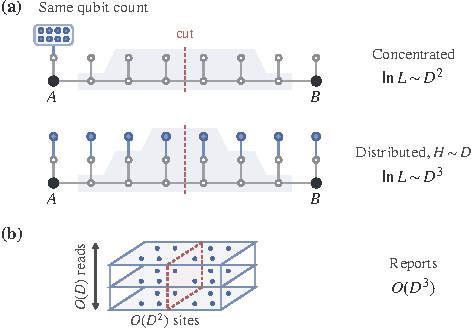
\includegraphics[width=\columnwidth]{Fig1.pdf}
\caption{\textbf{Where the measurement record can be protected.}
(a) The same eight ancillary sites, grouped at the source $A$ (top) or distributed along the path (bottom). Shading marks the sites within reach of an interior cut. Concentrating extra sites at the source gives quadratic logarithmic reach. Arms of height proportional to $D$ give cubic logarithmic reach. (b) Within depth $D$, the $O(D^2)$ sites near a path edge can each supply $O(D)$ reports.}
\label{fig:overview}
\end{figure}

Each joining measurement contributes one bit to each of two parities that determine the receiver's Pauli correction. If just one phase report is wrong, the receiver applies an extra $Z$ and obtains $\Phi^-$ instead of $\Phi^+$. The pair is still maximally entangled in that run, but the record leaves the receiver uncertain which Bell state it holds.

A measurement can act exactly as intended and still report the wrong bit. Errors in these mid-circuit reports affect feedback on quantum processors~\cite{Baumer2024,Koh2026,Smith2026}. An outcome can be protected by reading it several times or by encoding it in ancillary qubits~\cite{Hicks2022,Kim2025,Koh2026}, much as repeated syndrome measurements guide the corrections of a quantum code~\cite{Bombin2015,Harper2026}. On a 100-qubit chain, a baseline circuit gave Bell fidelity $0.39(1)$, while error detection gave $0.59(2)$ on accepted runs, above the threshold for certifying entanglement~\cite{Smith2026}. Could a sufficiently convincing record preserve endpoint entanglement at arbitrarily large distance for a fixed circuit depth?

We consider square-lattice devices with a bounded number of qubits per site and a unique path between the endpoints. Even with ideal gates and instantaneous classical feedback, readout errors alone give the endpoints a finite entangling reach. Beyond a distance $\exp[O(D^3)]$, any depth-$D$ circuit starting from a product state leaves the endpoints exactly separable in every reported record, however rare. One way to generate a noisy report is to return the true bit with probability $1-2p$ and an independent fair bit otherwise. If every report near a separating edge comes from a coin toss, that contribution to the endpoint state is separable. Within depth $D$ there are only $O(D^2)$ sites near the edge, each supplying $O(D)$ reports [Fig.~\ref{fig:overview}(b)]. A longer path crosses more disjoint regions of this kind. Counting them bounds the weight of the contribution that may still carry entanglement. To exclude even an arbitrarily weak entangled pair, we also use a product contribution near an endpoint.

Figure~\ref{fig:overview}(a) compares two layouts with the same number of qubits. An ancilla at the source can receive a distant report immediately, but only as a classical copy that carries the original error. An ancilla beside the measured qubit can instead copy the pointer's computational-basis value before readout and supply a fresh report of that value. Distributing the ancillas in arms of height proportional to $D$ therefore raises the attainable distance from $\exp[\Theta(D^2)]$ to $\exp[\Theta(D^3)]$ at the same number of qubits. On the resulting comb we implement a deterministic and nondestructive parity measurement of two distant data qubits with a single final round of feedforward. No arrangement of side networks in the square lattice can improve the cubic exponent as long as the endpoint path is unique. The same upper bound applies to modules joined in series by single links, with the number of such links in place of the distance, even when a module has many internal paths.

When measurement outcomes are known, the number of measured regions limits the speedup from feedback~\cite{Friedman2023}. Trinh \emph{et al.}\ proved that a chain supplied with one copy of a fixed full-rank two-qubit state per link has a finite entangling distance, even under adaptive local processing and postselection~\cite{Trinh2026}. Their bound depends on the smallest eigenvalue of the link state. In our setting the circuit can create pure Bell links and choose how much depth to spend protecting their measurement records. With multiple routes, redundant parity checks can protect cat-state order in two dimensions~\cite{Zhu2023,Chen2025}, and suitable networks can distribute Bell pairs below a noise threshold~\cite{Raussendorf2005,Choe2024,Harley2026}.

\smallskip
\paragraph*{Setting.}
Each cell of the interaction graph holds at most $b$ qubits. A layer acts on disjoint supports within cells or across neighboring cells. Every on-site binary measurement produces a true outcome and acts on the state accordingly, but the controller receives a report that is flipped independently with probability $0<p<1/2$. The reports of a run form its record, which the controller may use to adapt all later operations and to decide which runs to keep. The depth $D$ counts all gate and readout layers through the final correction, with at most one report per qubit and readout layer. Classical processing and communication are instantaneous, so that $D$ measures the quantum cost of making the record reliable. Ancillas start in a product state across cells. Our constructions use ideal gates and memories, whereas our upper bounds remain valid under additional local noise on gates and idle qubits.

Our benchmark task is the nondestructive measurement of the parity $Z_AZ_B$ of two data qubits at the endpoints, which may carry arbitrary inputs. With $P_s$ the projector onto the sector of parity $s$, the ideal instrument returns $s$ and preserves the coherence within each sector,
\begin{equation}
 \mathcal P_{ZZ}(\rho)=\sum_{s=0}^1 \ket{s}\bra{s}\otimes P_s\rho P_s .
 \label{eq:target-main}
\end{equation}
Measuring the two $Z$ values separately would give the right parity but destroy this coherence, on which lattice surgery relies~\cite{Horsman2012,Chamberland2022}. We quantify an implementation $\widetilde{\mathcal P}_{ZZ}$ by its operation error $\eps_{\rm op}=d_\diamond(\widetilde{\mathcal P}_{ZZ},\mathcal P_{ZZ})$, half the diamond-norm distance, which covers the returned bit as well as inputs entangled with a reference. On the input $\ket{++}$, the correction $X_B^s$ turns either ideal outcome into $\ket{\Phi^+}$, and the fidelity $F_{\rm corr}$ of this corrected Bell test obeys
\begin{equation}
 1-F_{\rm corr}\le \eps_{\rm op}.
 \label{eq:bell-bridge-main}
\end{equation}

\smallskip
\paragraph*{Reach on a single route.}
We focus on layouts with a single route between the endpoints, that is, on nearest-neighbor subgraphs of the square lattice with a unique simple path, of length $L$, between the two endpoint cells. We define two distances, both optimized over such layouts and over adaptive protocols of depth at most $D$. The entangling reach $L_{\rm ent}(D)$ is the largest distance at which a circuit acting on a product state leaves the endpoints entangled in at least one record of nonzero probability. Both the amount of entanglement and the probability of that record may tend to zero with distance. The deterministic reach $L_\eps(D)$ is the largest distance at which the parity measurement can be implemented with $\eps_{\rm op}\le\eps$ while keeping every run. Since an average Bell fidelity above $1/2$ requires an entangled pair in at least one record, Eq.~\eqref{eq:bell-bridge-main} gives $L_\eps(D)\le L_{\rm ent}(D)$ for $\eps<1/2$.

\begin{theorem}[Entangling reach at fixed depth]
\label{thm:time}
Fix $b\ge2$, $0<p<1/2$, and $0<\eps<1/2$. At each fixed depth, every record leaves the endpoints exactly separable beyond a finite distance, even after local filtering. For all sufficiently large $D$,
\begin{equation}
 \begin{aligned}
 \ln L_{\rm ent}(D)&=\Theta_b(\Lambda_p D^3),\\
 \ln L_\eps(D)&=\Theta_{b,\eps}(\kappa_p D^3),
 \end{aligned}
 \label{eq:optimal-reach}
\end{equation}
where $\Lambda_p=\ln[(1-p)/p]$ and $\kappa_p=-\ln[2\sqrt{p(1-p)}]$.
\end{theorem}

A single repeatedly measured bit illustrates the two information scales in Eq.~\eqref{eq:optimal-reach}. Majority decoding of $m$ reports has error at most $e^{-\kappa_pm}$. If all $m$ readings agree, the log-likelihood ratio in favor of the indicated bit is $m\Lambda_p$. The information ratio $\Lambda_p/\kappa_p$ grows as $4/(1-2p)$ as $p\to1/2$. Once $D$ is sufficiently large for the chosen detector, the ratio of the two logarithmic reaches is of order $\Lambda_p/\kappa_p$, with constants independent of $p$. The relative advantage of selection can therefore be large for a nearly uninformative detector, although the two reaches have the same cubic power of depth. The End Matter and Supplemental Material (SM) give the proof~\cite{SM}.

Restricting the layouts to combs with arms of height $H$ interpolates between the chain and this optimum. The corresponding reach obeys, uniformly in $H$ at fixed $p$ and $\eps$ (SM),
\begin{equation}
 \ln L_\eps(D,H)=\Theta\!\left(D^2\min\{D,H+1\}\right).
 \label{eq:height-main}
\end{equation}
Arms of fixed height retain the quadratic law of the chain, whereas arms of height of order $D$ attain the cubic law [Fig.~\ref{fig:reach}(a)]. More generally, optimizing over nearest-neighbor subgraphs of $\mathbb Z^\nu$ with a unique endpoint path gives logarithmic reach of order $D^{\nu+1}$ at fixed readout quality. The extra power counts the readout rounds available within a spatial neighborhood of order $D^\nu$ sites (SM).

\begin{figure}[t]
\centering
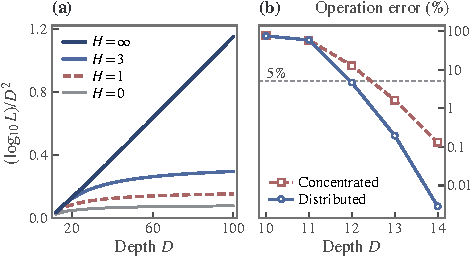
\includegraphics[width=\columnwidth]{Fig2.pdf}
\caption{\textbf{Reach and accuracy at fixed depth.}
(a) Achievable $\log_{10}L$ divided by $D^2$ for four arm heights at $p=1\%$ and $\eps=5\%$. (b) Lowest operation error within each family of simultaneous-readout schedules at $L=8399$ and $p=10\%$. The calculations use ideal gates and storage. Each layout has $33\,600$ resource sites and two data qubits. The $H=3$ comb reaches $5\%$ error in 12 layers. With height-one arms and the remaining sites in an idle source reservoir, the first qualifying schedule takes 13 layers. Each gate or readout layer counts once, including a SWAP layer.}
\label{fig:reach}
\end{figure}

\smallskip
\paragraph*{Why rare records cannot evade the bound.}
We fix the reported record and the controller's random seed, so that the local gates and measurement choices are specified. Consider the contribution in which every report within distance $D$ of a separating edge comes from a fair coin [Fig.~\ref{fig:overview}(b)]. These reports select no true outcomes. Summing over the outcomes leaves nonselective, trace-preserving maps in the neighborhood. Neither the endpoint observables nor any selected operation outside it can reach a crossing gate in backward evolution. Deleting the gates across the cut therefore preserves both the endpoint output and its branch probability~\cite{Friedman2023}. Product initialization then gives a separable contribution to the endpoint state.

A favorable record can make this event less likely. For either reported value, the coin part of the instrument dominates a fraction $p/(1-p)=e^{-\Lambda_p}$ of the reported map in completely positive order. The comparison survives subsequent operations chosen by the controller. Choose $K$ disjoint neighborhoods of separating edges, each containing neither endpoint and supplying at most $n$ reports. Within the observed branch the contribution with no fully replaced neighborhood has relative weight at most $(1-e^{-\Lambda_pn})^K$. Since this estimate is relative to the record itself, it applies equally to the rarest ones.

Even a small remainder can carry entanglement. Take the endpoints more than $2D$ apart and choose the $K$ neighborhoods outside the radius-$2D$ region around one endpoint. Replacing all reports in that endpoint region gives a product contribution that bounds the remainder in operator order. Its local factor at the endpoint stays fixed as we condition on replacements in the distant neighborhoods. Once the remainder is small enough, their sum lies in a separable neighborhood of the product contribution~\cite{Gurvits2002,Hanson2020}. If the endpoint region holds at most $n$ reports as well, we find for the endpoint qubits in every record $\boldsymbol y$ of nonzero probability
\begin{equation}
 Ke^{-\Lambda_pn}\ge\Lambda_pn+\ln3
 \quad\Longrightarrow\quad
 \rho_{AB\mid\boldsymbol y}\text{ is separable}.
 \label{eq:criterion-main}
\end{equation}
The End Matter proves this criterion for unequal report budgets on arbitrary interaction graphs.

On the square lattice, a path of length $L\gg D$ accommodates $K$ of order $L/D$ such neighborhoods with $n=O(bD^3)$ reports each, even if it folds back on itself. Equation~\eqref{eq:criterion-main} then gives $\ln L_{\rm ent}=O_b(\Lambda_pD^3+\ln(D+1))$. On a chain only $O(D)$ sites lie within reach of an edge, which gives the quadratic law. For transmission, place an untouched reference qubit at the source. Beyond the same distance every receiver branch is entanglement breaking~\cite{HSR2003}.

For a deterministic operation, the corrected Bell test measures fidelity averaged over all records. We replace the reports near one uniformly chosen cut by fair bits and withhold its position. Each modified circuit gives Bell fidelity at most $1/2$. When the cuts supply few reports, the mixture over their positions is hard to distinguish from the original circuit. A likelihood-ratio bound turns this into $2\kappa_pn\ge\ln[1+K(1-2\eps)^2]$ (SM), the deterministic upper bound in Eq.~\eqref{eq:optimal-reach}.

\smallskip
\paragraph*{Protecting outcome and coherence.}
Ancillary copies can accelerate the readout of a single system~\cite{Corlett2025}. On the comb we use them to protect the entire string of outcomes entering a remote correction. The comb is a chain whose sites carry ancillary arms [Fig.~\ref{fig:overview}(a)]. We divide the backbone chain into blocks, prepare a Bell pair across each block, and apply a Bell-basis transformation where neighboring blocks meet. Each interface then holds two computational-basis values on two pointer qubits, the bit and the phase outcome of its Bell measurement. Before any readout, we copy the two values with CNOT gates into the adjacent half-blocks and up their arms, where all copies are read in parallel. The first projective readout fixes the value shared by the copies of a bit, and every further report is an independent noisy reading of this value. All gates and bases are fixed in advance, and only the final correction uses the record. Its two Pauli bits are the parities of the majority-decoded values over all interfaces.

For $M$ interfaces with independent decoding errors of probability $q$ per bit, the corrected pair has Bell fidelity
\begin{equation}
 \Fe=\left[\frac{1+(1-2q)^M}{2}\right]^2 .
 \label{eq:resource-fidelity-main}
\end{equation}
The factor $(1-2q)^M$ is the probability of an even number of errors in a correction string minus the probability of an odd number. For fixed $0<q<1/2$ it tends to zero. A receiver that correctly decodes most interfaces still loses track of the accumulated correction. To keep the fidelity above $1/2$ by a fixed amount, the bit error must fall at least as fast as $1/M$. Since $q\le e^{-\kappa_pm}$ for $m$ readings, order $\ln M$ reports per bit suffice.

A block of $2\ell+2$ backbone sites whose arms are used up to height $h$, with every copy read $t$ times, provides $(\ell+1)(h+1)t$ reports per bit at a depth of $2\ell+h+t+O_{p,\eps}(1)$. Choosing $\ell$, $h$, and $t$ proportional to $D$ thus yields of order $D^3$ reports per bit and protects a number of interfaces exponential in $D^3$. If the extra qubits are instead concentrated at the source, no pointer of a distant block can reach them in time. Distant interfaces then keep the report budget of a chain, and the reach remains $\exp[\Theta(D^2)]$ however large the reservoir (SM). The cubic law uses repeated readout before the final correction. If only one readout round is allowed, the optimal depth is $\Theta(\ln L)$ on a chain and $\Theta(\sqrt{\ln L})$ on a tall comb (SM).

On a chain with three reports per bit at $p=1\%$, the averaged pair becomes separable at 1479 interfaces, whereas the best record remains entangled up to $427\,597$ interfaces [Fig.~\ref{fig:finite}(a)]. The ideal Bell bits in this chain have equal prior probabilities for zero and one. With three reports of such a bit, a two-to-one vote leaves posterior odds of $(1-p)/p$ for the majority value. Three agreeing reports give odds of $[(1-p)/p]^3$. The most favorable record combines the latter evidence at every interface. At $M=427\,597$, the probability that all $2M$ triples are unanimous is below $e^{-25\,000}$ (SM).

To measure the parity, each data qubit controls a CNOT onto its half of the protected pair, and both halves are read in $Z$. The reported parity is the XOR of the decoded endpoint outcomes in the corrected Bell frame. To see why this preserves coherence, take even data in the state $a\ket{00}+b\ket{11}$. The CNOTs leave both resource qubits alone in the first component and flip both in the second. Since $X\otimes X$ leaves $\Phi^+$ invariant, either component gives $00$ or $11$ with equal probability. The readout reveals the parity without distinguishing the two amplitudes. Only two endpoint decisions are added to the $2M$ interface decisions that determine the frame.

\begin{figure}[t]
\centering
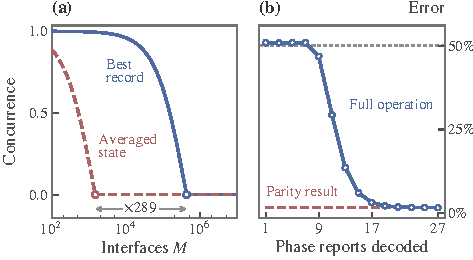
\includegraphics[width=\columnwidth]{Fig3.pdf}
\caption{\textbf{What averages and parity outcomes miss.}
(a) Endpoint concurrence~\cite{Wootters1998} for a chain with three reports per bit at $p=1\%$. Between the two marked thresholds the averaged state is separable and the best record is entangled. The probability of an entangled record falls from $48\%$ at $M=1479$ to $0.11\%$ at $M=2000$. (b) A fixed circuit acquires 27 reports per value at $L=8399$, $D=20$, and $p=10\%$. Only the decoder varies. Using more of its phase reports reduces the operation error while leaving the parity-result error unchanged.}
\label{fig:finite}
\end{figure}

A bit error in the frame reverses the returned parity. A phase error is invisible in the parity statistics because it changes only the relative phase within a sector. With an equal mixture of $\Phi^+$ and $\Phi^-$ as the resource, the parity statistics are correct for every input, and yet on $\ket{++}$ the even outcome leaves an incoherent mixture of $\ket{00}$ and $\ket{11}$. Repeating the parity check only confirms the first result. The phase correction uses information from the earlier measurements that joined the links. In our circuit the two residual errors are independent and the corrected Bell test distinguishes all four error patterns, so that
\begin{equation}
 1-\eps_{\rm op}=\Pr(\text{correct parity bit})\,\Pr(\text{no phase flip}).
 \label{eq:parity-phase-main}
\end{equation}
In Fig.~\ref{fig:finite}(b) we keep the circuit fixed and acquire all 27 reports per value. The bit decoder uses all 27 on every run. Increasing the number used for the phase correction lowers the operation error from $51\%$ to just above the $1.7\%$ error of the returned parity, whose statistics stay fixed. The change is visible in the corrected $XX$ correlation (SM).

\smallskip
\paragraph*{Speedup after protection.}
The Bell pair can be prepared before the data arrive. When the data are available from the start, we can instead apply the two endpoint CNOTs in the same layer as the interface CNOTs. Each end block has a free half-block for copies of its endpoint pointer. The endpoint and interface pointers can then be read in the same rounds, followed by a single phase correction.

At $L=8399$ and $p=10\%$, six copies of each pointer, each read three times, give an operation error of $4.65\%$ in 12 layers on the comb of Fig.~\ref{fig:reach}(b). With the same $33\,600$ resource sites, the concentrated layout retains height-one arms and leaves the remaining sites idle at the source. The height-one schedule first reaches the $5\%$ target in 13 layers. At that depth the operation errors are $0.20\%$ with distributed arms and $1.63\%$ with the source reservoir. The quadratic upper bound on the concentrated layout also covers protocols that put the reservoir to use (SM).

A circuit without measurements of depth $D<L/2$ has disjoint backward light cones at the two ends~\cite{BHV2006,FossFeig2023} and cannot pass the corrected Bell test from a product input. Coherent operation at this distance therefore needs at least 4200 layers, 350 times the depth of the protected measurement. When readout is slow compared with a gate, a larger copying region allows each round to collect more reports. The SM gives the optimal allocation for unequal layer times.

\smallskip
\paragraph*{Beyond a single route.}
In a line of modules, the cuts can be placed at the single links that all paths between modules must traverse (SM). On a general graph, even when no single edge separates the endpoints, the successive shells of cells at increasing graph distance from the source still cut every route. A device with $N$ physical qubits supplies at most $ND$ reports in depth $D$, a budget that all shells have to share. Applying the cut argument to disjoint shells (SM), we find that an entangled pair at graph distance $L$, in even a single record, requires
\begin{equation}
 ND^2=\Omega_p\!\left(L\ln L\right).
 \label{eq:hardware-main}
\end{equation}
Any layout with $O(L)$ qubits thus needs depth $\Omega_p(\sqrt{\ln L})$, which a chain attains for a reliable parity measurement. With a budget of order $wL$ qubits, combs remain optimal for $1\le w\lesssim(\ln L)^{1/3}$, at a depth of order $\sqrt{(\ln L)/w}$ (SM). At constant depth, Eq.~\eqref{eq:hardware-main} demands at least logarithmically many qubits per unit of graph distance. Harley and K\"onig achieve constant-depth Bell pairs on planar strips of polylogarithmic width below a noise threshold~\cite{Harley2026}, and the minimal width for a reliable constant-depth parity measurement remains open.

\smallskip
\paragraph*{Discussion and outlook.}
Suppose we keep the qubits of a comb in place and add horizontal couplings between neighboring arms. The resulting strip offers many routes at the same endpoint distance. Yet for $1\le w\lesssim(\ln L)^{1/3}$, Eq.~\eqref{eq:hardware-main} shows that the comb can leave all the added couplings idle and still implement the parity measurement in optimal asymptotic depth.

The upper bound allows noisy gates and storage on the same local supports. Their effect on the construction depends on where faults occur. A pointer flip before copying is inherited by every copy. Likewise, an independent phase fault of probability $g$ on each of $J$ prepared Bell links multiplies the corrected $XX$ correlation by $(1-2g)^J$, however accurately the pointers are read (SM). Achieving the cubic exponent in the presence of such faults calls for protection of the quantum links and data as well as their measurement records.

Rare readings in the tails of an ideal Gaussian detector can identify an outcome with arbitrarily high confidence, allowing constant-depth transmission at vanishing yield. With fixed finite digitization, if each occupied bin has positive probability for both outcomes, the evidence from any one reading is bounded and the single-route separability bound applies again (SM).

Classical feedback can carry a reported bit across the device in one step, along with any error it contains. A second reading must come from a qubit that still holds the outcome. Distributing such qubits along the path attains the cubic law for a reliable parity measurement that keeps every run. Even if a single entangled record would suffice, exceeding that law at fixed binary readout quality on the square lattice requires a second quantum route between the endpoints.




\bibliography{refs}

\onecolumngrid
\clearpage
\twocolumngrid
\section*{End Matter}
\paragraph*{A criterion for arbitrary interaction graphs.}
We prove Eq.~\eqref{eq:criterion-main} for unequal report budgets on an arbitrary interaction graph.
Let $d\le D$ count layers that can spread quantum support between cells,
and let $R\le bD$ bound the reports per cell, where $b$ is the fixed
local qubit capacity. Initialization is product across cells,
conditional on any initially available classical information.
Let $A$ be one final output qubit and $B$ any collection of output
registers outside the radius-$2d$ region around $A$.
Choose cuts that each separate $A$ from all of $B$. Their radius-$d$
neighborhoods $W_j$ contain every cell within graph distance
$d$ of an endpoint of a crossing edge. These neighborhoods must be
mutually disjoint, contain no output in $AB$, and lie outside the
radius-$2d$ region around $A$. Let $n_j$ and $n_0$ be deterministic
report budgets for these neighborhoods and the region around $A$,
respectively, valid for every reported record. Write
$Z_\alpha=\sum_j e^{-\alpha n_j}$ for the sum over interior cuts.
The neighborhood of $A$ is counted separately through $n_0$.

\begin{theorem}[Separability in every record]
\label{thm:range}
Under these conditions, the output on $AB$ is separable in every
positive-probability branch whenever
\begin{equation}
 Z_{\Lambda_p}\ge\Lambda_p n_0+\ln3.
 \label{eq:cut-range}
\end{equation}
The complete record may be retained. Record selection and local
filters on $A$ and $B$ preserve the conclusion.
\end{theorem}
Cuts with the smallest report budgets contribute most to $Z_{\Lambda_p}$. Each term bounds from below the relative weight of a cut with
uninformative reports. The right side accounts for the product
contribution supplied near $A$, which converts proximity to the
separable set into exact separability. Equation~\eqref{eq:criterion-main}
is the case in which no budget exceeds $n$.

\smallskip
\paragraph*{Reported instruments and cut deletion.}
For a binary on-site instrument $\{\mathcal M_0,\mathcal M_1\}$, whose
sum is trace preserving, the noisy map for report $y$ and its
fair-replacement contribution satisfy
\begin{equation}
 \begin{aligned}
 \mathcal A_y&=(1-p)\mathcal M_y+p\mathcal M_{1-y},\\
 \mathcal U_y&=p(\mathcal M_0+\mathcal M_1),\\
 e^{-\Lambda_p}\mathcal A_y&\preceq_{\rm CP}\mathcal U_y
       \preceq_{\rm CP}\mathcal A_y.
 \end{aligned}
 \label{eq:local-order}
\end{equation}
Here $\mathcal X\preceq_{\rm CP}\mathcal Y$ means
$\mathcal Y-\mathcal X$ is completely positive. Subtracting the fair
contribution from $\mathcal A_y$ leaves $(1-2p)\mathcal M_y$.
Subtracting $e^{-\Lambda_p}\mathcal A_y$ from $\mathcal U_y$ leaves
$p(1-2p)\mathcal M_{1-y}/(1-p)$.

Preassign independent report slots equal to each regional budget,
indexed by order of use, and assign independent slots to the remaining
reports. Each slot replaces the true outcome by a fair bit with
probability $2p$, including unused slots in the auxiliary probability
space. Independence makes this valid under adaptive scheduling.
Fix the reported record $\boldsymbol y$, replacement flags, fair bits, and controller
randomness $z$. Gates, bases, and schedules are fixed.
In a fully replaced cut neighborhood $W_j$,
summing true outcomes leaves trace-preserving maps after scalar report
weights are factored out. All selected,
non-trace-preserving maps lie outside it.

Let $\mathcal K_{\boldsymbol y,z}$ be the branch map with only $AB$ retained, and
$\widetilde{\mathcal K}_{\boldsymbol y,z}$ the map after deleting every gate across
the associated cut. Backward propagation of an observable $O_{AB}$ gives
\begin{equation}
 \mathcal K_{\boldsymbol y,z}^{\dagger}(O_{AB})
 =\widetilde{\mathcal K}_{\boldsymbol y,z}^{\dagger}(O_{AB}).
 \label{eq:adjoint}
\end{equation}
The adjoints of trace-preserving maps are unital. Every support insertion lies outside
$W_j$, at least $d+1$ cells from a crossing-edge endpoint, and cannot
reach a deleted gate in $d$ layers. The equality includes the identity,
so it preserves branch probabilities. After deletion, the initial
state and fixed evolution factor across the cut. The output contribution
is a positive product operator, and averaging over $z$ preserves separability.
Only trace preservation and the supports of the layers enter here, so
gates and idle steps may be replaced by arbitrary local channels.
A reference--input pair within one cell gives the analogous
entanglement-breaking statement for transmission. A related argument for
noisy quantum buses counts cuts where depolarization destroys the
entanglement shared by neighboring stations~\cite{Choe2024}.

\smallskip
\paragraph*{Replacement weight in a single record.}
Let $E_j$ denote full replacement in $W_j$ and $H$ an event determined
by flags outside $W_j$. For the reported branch map $\mathcal N_{\boldsymbol y}$, iteration
of Eq.~\eqref{eq:local-order} gives
\begin{equation}
 \mathcal N_{\boldsymbol y}^{H\cap E_j}
 \succeq_{\rm CP}e^{-\Lambda_p n_j}\mathcal N_{\boldsymbol y}^{H} .
 \label{eq:window-domination}
\end{equation}
Used slots give the local comparison and unused ones give $2p\ge e^{-\Lambda_p}$.
The regional padding makes the exponent $n_j$ valid for any fixed
budget that holds along every record. Applying the comparison
successively to disjoint neighborhoods yields
\begin{equation}
 \begin{gathered}
 \Pi=\prod_j(1-e^{-\Lambda_p n_j}),\\
 \mathcal N_{\boldsymbol y}=\mathcal E_{\boldsymbol y}+\mathcal G_{\boldsymbol y},\qquad
 0\preceq_{\rm CP}\mathcal G_{\boldsymbol y}
       \preceq_{\rm CP}\Pi\mathcal N_{\boldsymbol y} ,
 \end{gathered}
 \label{eq:branch-domination}
\end{equation}
where $\mathcal E_{\boldsymbol y}$ is entanglement breaking for transmission.
The corresponding preparation contribution is separable. No
independence of flags conditioned on $\boldsymbol y$ is assumed.

For transmission, retain $\boldsymbol y$ at the receiver and apply a
record-dependent trace-nonincreasing CP filter only there. For
preparation, allow record-dependent local filters on $A$ and $B$.
Summing accepted branches preserves both separability and CP order.
The normalized accepted state obeys
\begin{equation}
 \Fe^{\rm acc}\le\frac{1+\Pi}{2},\qquad
 \inf_{\sigma\in{\rm Sep}}\frac12
       \|\rho_{\rm acc}-\sigma\|_1\le\Pi .
 \label{eq:uniform-herald}
\end{equation}
This requires only positive acceptance probability. When it depends
on the input, the normalized accepted operation need not be a channel.


\begin{lemma}[A separable neighborhood]
\label{lem:one-sided-separable}
If $0\le X\le\Id/(\dim A)$, then
$\Id+X$ is separable across $A:B$, independently of the dimension of $B$.
\end{lemma}
\begin{proof}
For normalized Haar measure on pure states of $A$,
\begin{equation}
 \begin{aligned}
 \Id+X&=(\dim A)\int d\psi\,\ket\psi\bra\psi\otimes T_\psi,\\
 T_\psi&=\Id_B-\tr_A X
              +(\dim A+1)\langle\psi|X|\psi\rangle_A\ge0 .
 \end{aligned}
 \label{eq:strict-ball}
\end{equation}
The identity follows from the Haar second moment and positivity
from $\tr_A X\le\Id_B$. The operator-order condition involves only the dimension of $A$.
\end{proof}

\smallskip
\paragraph*{From proximity to exact separability.}
Fix the reported record and the controller's random seed. Write $\omega$
for the unnormalized endpoint state and $\omega_H$ for the contribution
from flag event $H$. Let $E_0$ denote full replacement in the radius-$2d$
neighborhood of $A$, with report budget $n_0$. Its contribution obeys
\begin{equation}
 e^{-\Lambda_p n_0}\omega\le\sigma_0\le\omega,\qquad
 \sigma_0:=\omega_{E_0}=\rho_A\otimes\sigma_B .
 \label{eq:strict-anchor}
\end{equation}
The causal past of $A$ shares no initial cell or gate with the pasts
of the distant outputs and outside selected maps. A shared initial cell
would require separation at most $2d$. A common gate in interaction layer
$j$ would require separation at most $2(d-j)+1$. The normalized factor
$\rho_A$ stays fixed under conditioning on outside flags because its cone
contains the same nonselective maps fixed by the record.

Let $E=\bigcup_{j\ge1}E_j$. The cut neighborhoods are disjoint from
the region defining $E_0$, so Eq.~\eqref{eq:window-domination} also
applies with $E_0$ fixed. Thus $\omega_{E_0\cap E}\ge(1-\Pi)\sigma_0$.
Both sides have the same $A$ factor, so their difference is a positive
product operator. The contribution from $E\setminus E_0$ is separable
by cut deletion. Grouping these two terms into a separable operator
$\sigma$ gives
\begin{equation}
 \begin{aligned}
 \omega &=(1-\Pi)\sigma_0+\sigma+\omega_{E^c},\\
 0\le\omega_{E^c}&\le\Pi\omega\le\Pi e^{\Lambda_p n_0}\sigma_0 .
 \end{aligned}
 \label{eq:strict-choi}
\end{equation}
The cut criterion gives $\Pi\le e^{-Z_{\Lambda_p}}\le e^{-\Lambda_p n_0}/3$.
If $\sigma_0=0$, then $\omega=0$. Otherwise restrict to its support
and conjugate locally by $\rho_A^{-1/2}\otimes\sigma_B^{-1/2}$, which
sends $\sigma_0$ to the identity. The transformed sum of the first and
last terms is $(1-\Pi)(\Id+X)$ with
$0\le X\le\Pi e^{\Lambda_p n_0}\Id/(1-\Pi)\le\Id/2$.
Lemma~\ref{lem:one-sided-separable} applies on this support since its
$A$ dimension is at most two. Undoing the congruence and adding
$\sigma$ proves separability. Averaging controller seeds, selecting
records, and applying endpoint filters preserve it.

\clearpage
\onecolumngrid
\begin{center}
\textbf{\large Supplemental Material for\\
Entangling reach of quantum circuits with noisy measurement records}\\[3pt]
\end{center}
\setcounter{equation}{0}
\setcounter{figure}{0}
\setcounter{table}{0}
\setcounter{section}{0}
\renewcommand{\theequation}{S\arabic{equation}}
\renewcommand{\thefigure}{S\arabic{figure}}
\renewcommand{\thetable}{S\arabic{table}}
\renewcommand{\theHtable}{S.\arabic{table}}
\renewcommand{\thesection}{S\arabic{section}}
\renewcommand{\theHequation}{S.\arabic{equation}}
\renewcommand{\theHfigure}{S.\arabic{figure}}
\renewcommand{\theHsection}{S.\arabic{section}}
\setcounter{secnumdepth}{2}

The End Matter bounds entanglement in each reported record. Section~\ref{sm:geometry}
uses that bound for the upper limit on reach and a random-cut comparison
for deterministic accuracy. The matching circuits use majority decoding
on all runs or select unanimous reports (Secs.~\ref{sec:comb-construction}
and~\ref{sm:unanimity}). Section~\ref{sec:finite-comb-schedules} gives the
integer schedules underlying Figs.~\ref{fig:reach} and~\ref{fig:finite}(b).

\FloatBarrier
\section{Remote operations and encoded endpoints}
\label{sm:operations}

\subsection{Nondestructive parity measurements}
The ideal remote parity instrument, including its returned classical bit, is
\begin{equation}
 \mathcal P_{ZZ}(\rho)
 =\sum_{s=0}^1\ket{s}\bra{s}_C\otimes P_s\rho P_s,
 \qquad P_s=\frac{\Id+(-1)^s Z_AZ_B}{2}.
 \label{eq:remote-parity-instrument}
\end{equation}
On $\ket{++}$, correcting the returned bit $s$ with $X_B^s$ gives
$\Phi^+$ for either ideal outcome. Thus Eq.~\eqref{eq:bell-bridge-main}
and Theorem~\ref{thm:range} bound the reach of the parity instrument,
including accepted operations whose normalized Bell test exceeds $1/2$.
This conclusion concerns the product-input test even if acceptance
depends on the input.

\begin{figure}[t]
\centering
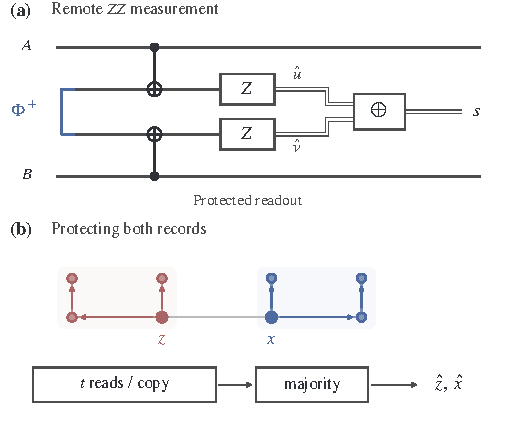
\includegraphics[width=0.55\textwidth]{FigS4.pdf}
\caption{\textbf{Protecting the parity result and the data coherence.}
(a) A shared Bell pair and endpoint-local CNOTs implement a nondestructive
$ZZ$ measurement. Protected $Z$ readouts of the resource qubits give decoded values $\hat u,\hat v$ and parity
$s=\hat u\oplus\hat v$. On $|++\rangle$, applying $X_B^s$ should
produce a Bell pair. (b) After each interface Bell-basis transformation,
the two pointers $z,x$ are copied into disjoint half-blocks and along
their arms. Each value has order $\ell\min\{\ell,H+1\}$ copies,
each read $t$ times, at duration $O(\ell+t)$. Parities of the decoded
values over all interfaces determine the resource corrections.}
\label{fig:protocol}
\end{figure}

For Fig.~\ref{fig:protocol}(a), prepare a corrected Bell pair on ancillas
$c_A,c_B$, apply $\mathrm{CNOT}_{A\to c_A}$ and $\mathrm{CNOT}_{B\to c_B}$,
then measure the ancillas in $Z$. The data Kraus operator for true
outcomes $u,v$ is $P_{u\oplus v}/\sqrt2$. Returning only $u\oplus v$
implements Eq.~\eqref{eq:remote-parity-instrument}. Related remote gates
also consume shared entanglement~\cite{Eisert2000}.

The resource produced by the protected wire is Bell diagonal. If its
Bell infidelity is $\delta$, its trace distance from $\Phi^+$ is exactly
$\delta$. Contractivity under the fixed instrument processor bounds the
induced half-diamond error by $\delta$, uniformly over data inputs and
spectator references. Read each endpoint pointer an odd number $m$ of
times and majority-decode. Each decision has error
$q_m(p)\le e^{-\kappa_p m}$, independently of its true value. A union
bound on the two endpoint errors gives
\begin{equation}
 d_\diamond(\widetilde{\mathcal P}_{ZZ},\mathcal P_{ZZ})
 \le\delta+2q_m(p).
 \label{eq:remote-parity-error}
\end{equation}
This includes the returned register $C$. Choosing $\delta\le\eps/2$ and
$q_m(p)\le\eps/4$ adds only $O_{p,\eps}(1)$ endpoint layers, using
nondemolition readout or the fresh probes of Sec.~\ref{sm:wire-upper}.

The two resource errors have distinct effects. With resource
$(\Id\otimes X^xZ^z)\ket{\Phi^+}$, the data Kraus operator for true
outcomes $u,v$ is
$K_{uv}^{xz}=(-1)^{zu}Z_A^zP_{u\oplus v\oplus x}/\sqrt2$.
Thus $x$ changes the returned parity and $z$ introduces a phase error
within its sector. An equal mixture of $\Phi^+$ and $\Phi^-$ gives the
ideal parity probabilities for every input, but separable conditional
outputs on $\ket{++}$.
For any Bell-diagonal resource and ideal endpoint reports, the
half-diamond error equals the Bell infidelity. Contractivity gives the
upper bound. On input $\ket{++}$ the correction $X_B^s$ yields four
orthogonal Bell outputs for the four resource errors, attaining the bound. For the wire with
$M$ actual swapping interfaces, write $\lambda=(1-2q)^M$ and let each
endpoint decoder err independently with probability $r_{\rm e}$. The same argument
gives the exact full-instrument error
\begin{equation}
 d_\diamond(\widetilde{\mathcal P}_{ZZ},\mathcal P_{ZZ})
 =1-\frac{[1+\lambda(1-2r_{\rm e})^2](1+\lambda)}4.
 \label{eq:parity-exact-error}
\end{equation}
The output register contains only the decoded parity.

Remote CNOT has the same fixed-accuracy scaling. Its action on
$\ket{+0}$ gives the Bell-test lower bound. For the upper bound, use
$\mathrm{CNOT}_{A\to c_A}$, a $Z$ measurement of $c_A$ and the corresponding
$X_{c_B}$ correction, followed by $\mathrm{CNOT}_{c_B\to B}$, an $X$ measurement
of $c_B$, and the corresponding $Z_A$ correction~\cite{Eisert2000}.
Protect the two reports as above. Preparing the Bell resource before
coupling to unknown data also makes the unanimous-report resource
selection input independent. It supplies accepted parity measurements
and remote CNOTs with the same distance exponents.

These transfers compare tasks at fixed $p$ and fixed accuracy. The
uniform detector and unequal-duration results below are stated for
transmission, whose optimum is denoted by $\Dopt$ or $\Topt$.
The flagged parity instrument must additionally acquire its returned
bit, whereas coherent SWAP transmission can use no readout at all.

\subsection{Pre-encoded endpoint blocks}
\label{sm:encoded-endpoints}
Allow arbitrary initial encoding within two confined endpoint blocks.
It suffices that the initial state factor across every chosen interior
cut. In particular, the two blocks may contain arbitrary independent
encoded states while the intervening cells start in a product state.
Choose disjoint cut neighborhoods containing no cell of either block.
This places every block cell at least $d+1$ from each crossing-edge endpoint. For a
fully replaced neighborhood, Eq.~\eqref{eq:adjoint} still deletes the
cut, leaving a separable contribution across the endpoint blocks.
Initial entanglement within a block does not affect this factorization.

The comparison in Eq.~\eqref{eq:branch-domination} therefore gives, for
every reported branch, $\omega_{\boldsymbol y}=E_{\boldsymbol y}+G_{\boldsymbol y}$ with $E_{\boldsymbol y}$ separable and
$0\le G_{\boldsymbol y}\le\Pi\omega_{\boldsymbol y}$, where
$\Pi=\prod_j(1-e^{-\Lambda_p n_j})$.
Any record-dependent joint decoder or trace-nonincreasing local filter
within either endpoint block preserves this comparison and separability.
After selecting and normalizing any positive-probability set of records,
the nonseparable remainder has relative trace at most $\Pi$.
The decoded two-qubit Bell fidelity consequently obeys
\begin{equation}
 \mathcal F_{\rm log}^{\rm acc}\le
 \frac12\left[1+\prod_j(1-e^{-\Lambda_p n_j})\right].
 \label{eq:encoded-endpoints}
\end{equation}

An accurate logical parity measurement on
$\ket{+_{\rm L}}\ket{+_{\rm L}}$, followed by the reported logical
correction, or logical CNOT on $\ket{+_{\rm L}}\ket{0_{\rm L}}$, must
produce logical Bell fidelity at least $1-\eps$.
Since $\Pi\le e^{-Z_{\Lambda_p}}$, this requires
\begin{equation}
 \sum_j e^{-\Lambda_p n_j}\le -\ln(1-2\eps).
 \label{eq:encoded-report-cost}
\end{equation}
Packing interior cuts with the same chain or comb capacities gives
the corresponding fixed-accuracy duration lower bounds. The distance
is the gap between the blocks. The bound allows free joint decoding within each block under the
assumed factorization across interior cuts. Encoding and logical
operations may increase the depth for a particular endpoint code.

\paragraph*{Exact separability after logical decoding.}
For a strict statement, assume the initial state has the form
$\rho_{\mathcal A}\otimes\rho_{\mathcal B}\otimes
\bigotimes_{v\notin\mathcal A\cup\mathcal B}\rho_v$,
where $\mathcal A,\mathcal B$ are the full retained endpoint blocks
and $\operatorname{dist}(\mathcal A,\mathcal B)>2d$.
Their internal states are unrestricted. Replace all reports in
$N_{2d}(\mathcal A)$, with budget $n_0$, and choose the separating
cut neighborhoods outside this region and disjoint from both blocks.
At fixed reported record and controller seed, the backward pasts of
$\mathcal A$ and of all distant outputs and outside selected maps share
no gate or initial factor. Neither past reaches the other block's initial state, and the
remaining initial factors are products across cells.
The replaced region gives $\sigma_0=\tau_{\mathcal A}\otimes\sigma_{\mathcal B}$.
Here $\tau_{\mathcal A}$ is the output of the nonselective maps in the
block's past for the fixed record and seed. Conditioning on flags
outside the region leaves this factor unchanged. Equations~\eqref{eq:strict-anchor}
and~\eqref{eq:strict-choi} apply to the two blocks.

Apply a record-dependent CP decoder from $\mathcal A$ to one logical
qubit to every term in the decomposition. It preserves CP order,
product structure, and separability, and the decoded anchor factor has
rank at most two. If that factor vanishes, domination makes the whole
decoded branch vanish. Otherwise the same support restriction and Haar
identity~\eqref{eq:strict-ball} give exact separability whenever
$\Pi\le e^{-\Lambda_p n_0}/3$, hence under Eq.~\eqref{eq:cut-range} in the End Matter.
Any local decoder or filter on $\mathcal B$ preserves the conclusion.
This proves failure of the logical product-input Bell test in each
accepted record. It does not assert that the two-input parity instrument
is itself entanglement breaking on already entangled inputs.
For a block occupying $u$ consecutive chain cells, the enlarged
anchor has budget $n_0\le R(u+4d)$.

\FloatBarrier
\section{Geometry and ancillary placement}
\label{sm:geometry}
\subsection{Report budgets and refinements of the cut bound}
We use the interaction-depth refinement proved in the End Matter,
with $d\le D$ and at most $R\le bD$ reports per cell. The binary
Chernoff information is $\kappa_p=-\ln[2\sqrt{p(1-p)}]$.
For $K$ disjoint cut neighborhoods with budgets $n_j\le n$,
Eq.~\eqref{eq:uniform-herald} gives
$\Pi\le\exp(-K e^{-\Lambda_p n})$.
Accepted fidelity $1-\eps>1/2$ therefore requires
$n\Lambda_p\ge\ln K-\ln[-\ln(1-2\eps)]$.
The exact product bound also gives $n\Lambda_p\ge-\ln(2\eps)>0$.

For $K\ge2$ disjoint neighborhoods with at most $n$ reports each,
fixed-accuracy transmission requires
\begin{equation}
 n\gtrsim_\eps
 \begin{cases}
 \ln K/\kappa_p,&\text{deterministic},\\
 \ln K/\Lambda_p,&\text{postselected}.
 \end{cases}
 \label{eq:two-information-costs}
\end{equation}
The constants are independent of $p$. The End Matter gives the
arbitrary-yield bound. We derive the deterministic bound below. The constructions match their
detector dependence on a chain. Majority decoding and unanimous-record selection
have the respective binary discrimination exponents $\kappa_p$ and
$\Lambda_p$~\cite{Chernoff1952,DAnjou2021,Regula2024}.
They vanish quadratically and linearly, respectively, as $p\to1/2$.


The cut regions are fixed before the run. The budgets in
Theorem~\ref{thm:range} are fixed upper bounds on all
reported histories. They may be smaller than $R$ times the number of
cells in a region. Preassign that many independent slots to each
region and consume them in temporal order, breaking ties in a fixed order. Adaptive choices of the measured cells do not
change the reporting law. This justifies the regional padding in the
End Matter without assuming a fixed schedule.

The CP comparison also controls more general events in the auxiliary
replacement flags. Fix a record $\boldsymbol y$ and write its CP contributions
as $\mathcal N_{\boldsymbol y}^z$, with $z_i=1$ denoting replacement at slot $i$.
For every configuration of the other flags, the local inequality gives
$\mathcal N_{\boldsymbol y}^{(1,z_{-i})}\succeq_{\rm CP}
e^{-\Lambda_p}[\mathcal N_{\boldsymbol y}^{(0,z_{-i})}+\mathcal N_{\boldsymbol y}^{(1,z_{-i})}]$.
For any event $E$ decreasing in the replacement flags,
\begin{equation}
 \mathcal N_{\boldsymbol y}^E\preceq_{\rm CP}
       \Prb_{\rm iid}(E)\mathcal N_{\boldsymbol y},
 \label{eq:flag-domination}
\end{equation}
where $\Prb_{\rm iid}$ denotes independent replacement with probability
$e^{-\Lambda_p}$ at each slot. To prove this without operator-valued conditional probabilities,
apply every Choi-space vector $v$ to define the positive scalar measure
$\mu_v(z)=\langle v|J(\mathcal N_{\boldsymbol y}^z)|v\rangle$.
After normalization, each sequential conditional replacement probability
is at least $e^{-\Lambda_p}$. Shared independent uniform random numbers therefore
couple its flags coordinatewise above independent Bernoulli($e^{-\Lambda_p}$)
flags. A decreasing event has smaller probability. The resulting
inequality for every $v$ is precisely Eq.~\eqref{eq:flag-domination}.
The zero-mass case is immediate. Unused slots satisfy the same local
comparison since $2p\ge e^{-\Lambda_p}$. To obtain a cut bound,
the complementary event must separate the outputs.

\paragraph*{Deterministic comparison.}
Compare the original channel with a mixture in which one uniformly
chosen cut neighborhood supplies only fair reports. We bound their
distance by the second moment of the mixture likelihood ratio, a
method also used in quantum state certification~\cite{ChenLiODonnell2022}.
Pad each of $K$ disjoint neighborhoods to $n$ independent
Bernoulli($p$) error slots. Their product law is $\mu$.
For a fixed error array $e$, the adaptive protocol defines a
trace-preserving channel $\channel_e$, including its complete
reported record. Thus $\channel=\mathbb E_\mu\channel_e$.
Let $\mu_j$ replace the error bits in neighborhood $j$ by independent
fair bits. The used reports there become independent of their true
outcomes, so $\mathcal S_j=\mathbb E_{\mu_j}\channel_e$ is entanglement
breaking. Unused slots integrate out.

The likelihood ratios $\mathcal L_j=d\mu_j/d\mu$ are independent, with
$\mathbb E_\mu\mathcal L_j=1$ and
$\mathbb E_\mu\mathcal L_j^2=[4p(1-p)]^{-n}=e^{2\kappa_p n}$.
For $\mathcal S=K^{-1}\sum_j\mathcal S_j$, the triangle inequality
and $\|\channel_e\|_\diamond=1$ give
\begin{equation}
 \begin{aligned}
 d_\diamond(\channel,\mathcal S)
 &\le\frac12\mathbb E_\mu\left|1-\frac1K\sum_j\mathcal L_j\right|\\
 &\le\frac12\sqrt{\frac{e^{2\kappa_p n}-1}{K}} .
 \end{aligned}
 \label{eq:statistical-eb}
\end{equation}
The comparison is uniform over reference-entangled inputs.
Since $\mathcal S$ is entanglement breaking, fidelity at least
$1-\eps$ requires
\begin{equation}
 2\kappa_p n\ge\ln[1+K(1-2\eps)^2].
 \label{eq:detector-resource}
\end{equation}
This proves the deterministic part of Eq.~\eqref{eq:two-information-costs}.
For unequal budgets the mixing weights can depend on the cut.
The likelihood ratios for separate regions fluctuate independently
with variances $v_j=e^{2\kappa_p n_j}-1$.
For normalized weights $w_j$, Cauchy--Schwarz gives
$(\sum_j w_j^2v_j)(\sum_j v_j^{-1})\ge1$ when all $v_j>0$.
Mixing the entanglement-breaking channels with $w_j\propto 1/v_j$
attains equality and gives
\begin{equation}
 \inf_{\mathcal S\in\mathrm{EB}}
 d_\diamond(\channel,\mathcal S)
 \le\frac{1}{2\sqrt{\displaystyle\sum_j
                      (e^{2\kappa_p n_j}-1)^{-1}}}.
 \label{eq:weighted-statistical-eb}
\end{equation}
If some $n_j=0$, the channel is already entanglement breaking and the
right side is zero. For positive budgets the sum in the denominator is at
least $Z_{2\kappa_p}$, so $1/(2\sqrt{Z_{2\kappa_p}})$ is a simpler upper
bound. Equation~\eqref{eq:weighted-statistical-eb} retains the stronger
finite-size estimate and recovers Eq.~\eqref{eq:statistical-eb} for equal budgets.

Finally, a bounded output region $A$ obeys the same
strict graph criterion with $\ln(\dim A+1)$ in place of $\ln3$.
The anchor is the radius-$2d$ neighborhood of the whole output region.
Lemma~\ref{lem:one-sided-separable} gives separability of
$\Id+X$ for $0\le X\le\Id/(\dim A)$, independently of the receiving
dimension. Thus the End Matter applies with
$\Pi\le e^{-\Lambda_p n_0}/(\dim A+1)$. Each cut must separate the entire
receiving region, not merely one of its output sites.

\paragraph*{Repeated preparations and purification.}
Tensor products of independently completed separable outputs remain
separable under local operations and classical communication, including
entanglement distillation. Concurrent preparations, continued use of
intermediate quantum memory, and additional purification steps must
instead be charged to the combined protocol. The graph bound applies to the total depth and report budgets for
preparations starting from a product state.

\subsection{Finite-height combs: exact geometric counts}
\label{sec:comb-proof}

The comb has vertices $(x,y)$ with $0\le x\le L$ and $0\le y\le H$.
Edges join $(x,y)$ to $(x,y+1)$ along each arm and $(x,0)$ to
$(x+1,0)$ along the backbone.  It is a degree-three tree embedded
with nearest-neighbor edges in a square lattice.  The two endpoints
of interest are $(0,0)$ and $(L,0)$.
No horizontal connections between different arms are available.

For a backbone edge the number of cells in its radius-$d$ neighborhood
is at most
\begin{equation}
 \begin{split}
 v_d(H)&=2\sum_{r=0}^{d}\min\{H+1,r+1\}\\
 &=\begin{cases}
 (H+1)(2d-H+2),&H\le d,\\
 (d+1)(d+2),&H\ge d .
 \end{cases}
 \end{split}
 \label{eq:comb-window}
\end{equation}
For the anchor around a backbone site, the corresponding bound is
\begin{equation}
 \begin{split}
 u_d(H)&=\min\{H+1,2d+1\}
             +2\sum_{r=1}^{2d}\min\{H+1,r\}\\
 &=\begin{cases}
 (H+1)(4d-H+1),&H\le2d,\\
 (2d+1)^2,&H\ge2d .
 \end{cases}
 \end{split}
 \label{eq:comb-anchor}
\end{equation}
These are the exact counts for an infinite backbone.  Endpoint
boundaries only reduce them.
Spacing cut edges by $2d+2$ along the backbone gives disjoint windows.
Excluding the anchor and endpoint windows still leaves
$K\ge L/[8(d+1)]$ when $L\ge16(d+1)$.
Consequently, the endpoint output is separable in every reported
branch if
\begin{equation}
 L\ge
 \max\!\left\{16(d+1),
 8(d+1)[\Lambda_pR u_d(H)+\ln3]\,
                 e^{\Lambda_pR v_d(H)}\right\}.
 \label{eq:comb-exact-separability}
\end{equation}

At fixed local reporting capacity, $d\le D$ and $R\le bD$.
The volumes in Eqs.~\eqref{eq:comb-window} and
\eqref{eq:comb-anchor} are of order
$(d+1)\min\{d+1,H+1\}$, uniformly in $H$.
Thus any protocol producing an entangled endpoint pair, or a
non-entanglement-breaking transmission branch, must satisfy
$\ln L=O_{p,b}(D^2\min\{D,H+1\})$ in the sublinear-duration regime.
If $L<16(d+1)$ the required lower bound is immediate instead.
The resulting bound is
\begin{equation}
 D=\Omega_{p,b}\!\left(
 \max\left\{(\ln L)^{1/3},
       \sqrt{\frac{\ln L}{H+1}}\right\}\right).
 \label{eq:comb-depth-lower}
\end{equation}
It holds at arbitrary positive postselection yield.

\subsection{Optimality among square-lattice layouts with a unique path}
\label{sec:square-unique-path}
\begin{corollary}[Optimal range with a unique connecting path]
Let $G$ be any nearest-neighbor subgraph of the square lattice, with a
unique simple path of length $L$ between prescribed endpoint cells.
Assume product initialization across cells, fixed local qubit capacity,
and at most $bD$ reports per cell in duration $D$. At fixed
$0<p<1/2$, every reported two-qubit endpoint state is separable when
$\ln(L+1)>C_{p,b}(D+1)^3$, for a constant independent of $G$.
The largest entangling range over this class is therefore
$\exp[\Theta_{p,b}(D^3)]$. Tall combs attain this order, also for
complete parity operations at fixed accuracy.
\end{corollary}

\begin{proof}
Write the unique path as $v_0,\ldots,v_L$. Every path edge is a bridge,
and any connected component off the path meets it at most once.
Otherwise a second simple endpoint path would exist. Graph distances
between path vertices therefore equal their distances along the path,
even when its embedding bends back on itself.

For $D\ge1$, choose edges $(v_k,v_{k+1})$ with
$k=3D+1+j(2D+2)$ and $k\le L-D-2$. Their radius-$D$ neighborhoods
are disjoint, avoid the endpoints, and lie outside the radius-$2D$
neighborhood of $v_0$. When $L\ge16(D+1)$, there are at least
$K\ge L/[8(D+1)]$ such cuts. A radius-$D$ graph ball lies inside a
square-lattice Manhattan ball, which has $1+2D(D+1)$ cells.
Consequently each cut neighborhood has at most $4(D+1)^2$ cells,
and the source neighborhood has at most $8(D+1)^2$ cells.

Put $x=8b\Lambda_pD(D+1)^2$. Both $\Lambda_p n_j$ and
$\Lambda_p n_0$ are bounded by $x$. Theorem~\ref{thm:range} then
implies separability whenever $Ke^{-x}\ge x+\ln3$. In particular,
the explicit sufficient distance
\begin{equation}
 L\ge16(D+1)(x+\ln3)e^x,
 \qquad x=8b\Lambda_pD(D+1)^2
 \label{eq:square-unique-path-range}
\end{equation}
has logarithm $O_{p,b}((D+1)^3)$. All bounds hold within every
reported branch and survive local endpoint filters. The construction in Sec.~\ref{sec:comb-construction} attains the matching reach.
\end{proof}

For any fixed spatial dimension $\nu\ge1$, the same packing argument
applies to nearest-neighbor subgraphs of $\mathbb Z^\nu$ with a unique
endpoint path. Both a cut neighborhood and the endpoint neighborhood
contain $O_\nu((D+1)^\nu)$ cells, each supplying at most $bD$ reports.
Equation~\eqref{eq:cut-range} thus gives $\ln L=O_{p,b,\nu}(D^{\nu+1})$
for any entangled endpoint branch. To attain this exponent, attach a
transverse $(\nu-1)$-dimensional box of side $\ell$ to each backbone
site, with edges between successive boxes only at their roots. The block
circuit copies each interface value along its own half-block and into
the attached boxes, filling $\Theta_\nu(\ell^\nu)$ sites in $O_\nu(\ell)$
layers. With $\ell$ readout rounds, majority decoding suppresses the
error per value exponentially in $\ell^{\nu+1}$. Taking $\ell$ proportional
to $D$ with a sufficiently small prefactor attains
$\ln L=\Omega_{p,\eps,\nu}(D^{\nu+1})$ for the complete parity
measurement at fixed accuracy. For $\nu=1$ each box is a single site.

\paragraph*{Readout dependence of the two reaches.}
For fixed target error $0<\eps<1/2$, the two reaches in
Theorem~\ref{thm:time} obey
\begin{equation}
 \ln L_\eps(D)=\Theta_{b,\eps}(\kappa_pD^3),\qquad
 \ln L_{\rm ent}(D)=\Theta_b(\Lambda_pD^3).
 \label{eq:two-reach-costs}
\end{equation}
The comparison constants are independent of $p$. It suffices that $D$
exceed an absolute constant and $\kappa_pD^3\ge C_\eps\ln(D+1)$ for
sufficiently large $C_\eps$. Every fixed $0<p<1/2$ meets this condition
at large depth.

For the deterministic upper bound, apply the random-cut comparison
of Eq.~\eqref{eq:statistical-eb} to the corrected $\ket{++}$ test.
Each modified circuit gives separable endpoints and hence Bell fidelity
at most $1/2$. The likelihood-ratio estimate for this fixed input gives
$K(1-2\eps)^2\le e^{2\kappa_p n}-1$, with at most
$n=4bD(D+1)^2$ reports per cut neighborhood. The packing bound above
then gives $\ln L\le O_{b,\eps}(\kappa_pD^3+\ln(D+1))$, also when
$L<16(D+1)$. Equation~\eqref{eq:square-unique-path-range} gives the
corresponding upper bound $O_b(\Lambda_pD^3+\ln(D+1))$ for any
entangled record. Since $\Lambda_p\ge\kappa_p$, the stated condition
absorbs both logarithmic terms.

For achievability choose $\ell=h=t=\lfloor(D-5)/4\rfloor$ in
Eq.~\eqref{eq:comb-fixed-distance-schedule}, with $J$ equal blocks
and $L+1=J(2\ell+2)$. The schedule fits within $D$ layers and gives
$m=\Theta(D^3)$ reports per bit, counting the endpoint bits as well.
Majority decoding has complete parity-measurement error at most
$2Je^{-\kappa_p m}$. Taking $J=\lfloor\eps e^{\kappa_p m}/2\rfloor$
gives the first lower bound. For the second, retain the Bell endpoints
without coupling data to them. Condition on a complete record in which
all reports of each interface bit agree. The corrected pair then
has infidelity at most $2(J-1)e^{-\Lambda_p m}$ by
Eq.~\eqref{eq:unanimity-bit}. Such records have positive probability.
Taking $J=\lfloor e^{\Lambda_p m}/8\rfloor$ leaves the pair entangled.
Thus the ratio of the two logarithmic reaches is of order
$\Lambda_p/\kappa_p$ in the stated regime. This information ratio tends
to two as $p\to0$ and grows as $4/(1-2p)$ as $p\to1/2$. The geometric
prefactors in Eq.~\eqref{eq:two-reach-costs} are not fixed by these limits.

The hypothesis is a unique simple path. A second, longer route would
already invalidate the bridge argument. Planarity alone also permits
the exponentially growing trees of Sec.~\ref{sec:branching-tree}.

The same argument bounds the number of unavoidable edges even when
the endpoint path is not unique. Let $m$ count the bridges whose
removal separates the two endpoints. Contracting the connected
components left after deleting bridges gives a tree, with these $m$
bridges ordered along its endpoint path. Bridge indices differing by
$2D+2$ have endpoint sets at graph distance at least $2D+1$.
Omitting the first $3D+1$ and last $D+1$ bridges leaves the same
packing bound $K\ge m/[8(D+1)]$ when $m\ge16(D+1)$.
Equation~\eqref{eq:square-unique-path-range} therefore remains a
sufficient separability condition with $m$ in place of $L$.
This covers large two-dimensional modules joined in series by single
links, even when each module contains many internal routes.

\paragraph*{A qubit budget on arbitrary interaction graphs.}
Let $N$ be the total number of physical qubits and $L$ the endpoint graph distance.
At fixed $0<p<1/2$, generating an entangled endpoint pair in even one
reported branch requires $ND^2=\Omega_p(L\ln(L+1))$. To see this, group
the cells by their graph distance from the first endpoint. A gate crosses
at most one level. When $L\gg D$, the interior levels contain $2k$
disjoint shells of $2D+2$ consecutive levels each, with $k$ of order
$L/(D+1)$. The middle of each shell cuts every route to the receiver.

Assign $D$ potential report slots to each qubit. The aggregate shell
budget is at most $ND$. Choose the shell of smallest budget among the
first $k$ as the anchor and use the last $k$ as separating shells.
Put $x=\Lambda_p ND/k$. The anchor budget $n_0$ obeys
$\Lambda_p n_0\le x$. For the outer shell budgets $n_j$, Jensen's
inequality gives $\sum_j e^{-\Lambda_p n_j}\ge k e^{-x}$.

Here the anchor is an interior cut. Fix the actual record and controller
seed. With all reports in the anchor replaced, deleting its crossing
gates leaves a product branch operator because the initial state factors
across the cut and the frozen maps act separately on its two sides. Conditioning
further on replacement flags in the outer shells changes only its
receiver-side factor, since all those flags lie beyond the anchor.
Thus the same product component and separable-neighborhood argument as in
Eqs.~\eqref{eq:strict-anchor} and~\eqref{eq:strict-choi} applies.
In particular, $k e^{-x}\ge x+\ln3$ suffices for exact separability.
An entangled branch therefore requires $x=\Omega(\ln k)$ for large $k$.
For $1\le D\le\sqrt L$, this gives the claimed hardware bound. For
$D>\sqrt L$ it follows already from $N\ge L+1$ on the occupied graph.
At fixed accuracy, the comb of height of order $w$ uses $O(wL)$ qubits
and attains this lower bound when $1\le w\le C[\ln(L+1)]^{1/3}$ for
fixed $C$, by Eq.~\eqref{eq:comb-depth-optimal}.

\subsection{Matching comb construction}
\label{sec:comb-construction}

First construct an endpoint Bell pair with one physical qubit per
comb vertex.  Choose an integer $\ell$ and put
$J=\lfloor(L+1)/(2\ell+2)\rfloor$.
Partition the backbone into $J$ consecutive, disjoint intervals.
The first $J-1$ intervals have $2\ell+2$ vertices, and the last
contains all remaining vertices, between $2\ell+2$ and $4\ell+3$.
Their outer endpoints are the prescribed sites $(0,0)$ and $(L,0)$.
In the asymptotic regime used below, $J\ge2$.

Prepare a Bell pair between the two endpoints of each interval in
parallel.  A local Bell pair followed by swaps moves one half to
the far endpoint in $O(\ell)$ depth, leaving all interior transport
qubits in $|0\rangle$.
The right endpoint of one interval and the left endpoint of the next
are adjacent.  Apply a Bell-basis transformation to each such pair.
Its two qubits now hold computational-basis values specifying the
two eventual Pauli corrections.

Copy the left value leftward through the $\ell$ nearest interior
vertices of its interval, and the right value rightward through the
$\ell$ nearest interior vertices of the following interval.
The two groups occupy disjoint halves, leaving any surplus vertices
in the final interval unused.
Then copy each occupied backbone value upward along its arm to
height $\min\{\ell,H\}$.
Both stages run in parallel across all interfaces in $O(\ell)$ depth.
Neither final endpoint is copied or measured.
Each Bell value has
$(\ell+1)(\min\{\ell,H\}+1)$ identical computational-basis copies,
including its original pointer.

Keep the largest odd number $N$ of these copies, and choose an odd
number $t$ of repeated same-basis readouts of each retained copy.
Discarding at most one copy gives
$N\ge(\ell+1)(\min\{\ell,H\}+1)/2$.
Majority decoding therefore has error
$q\le e^{-\kappa_pNt}$ per Bell value.
The exact parity formula, or a union bound over the $2(J-1)$ values,
gives
\begin{equation}
 \begin{split}
 1-\Fe&\le2(J-1)e^{-\kappa_pNt},\\
 D&=O(\ell+t).
 \end{split}
 \label{eq:comb-explicit-upper}
\end{equation}
Same-basis nondemolition readout gives fresh, independently corrupted
reports of the same stored value.

Take $\ell$ and $t$ of the same order, proportional to
\[
 \max\!\left\{
 \left[\frac{\ln(4L/\eps)}{\kappa_p}\right]^{1/3},
 \sqrt{\frac{\ln(4L/\eps)}
              {\kappa_p(H+1)}},\,1\right\}.
 \]
Then $\kappa_pNt\ge\ln(4L/\eps)$ after increasing the fixed
proportionality constant, and the Bell-pair error is at most $\eps/2$.
Integer rounding and the odd-subset convention change only constants.
For fixed $p,\eps$ and sufficiently large $L$, this choice has
$\ell=o(L)$, as required by the interval partition.

For transmission, add an input qubit in the source cell and perform a
local Bell measurement onto the prepared pair. A fixed number of rereads
limits the error of its two injection bits to $\eps/2$. This adds
$O_{p,\eps}(1)$ layers and gives Bell fidelity at least $1-\eps$.

For the parity operation, add a data qubit in each endpoint cell and
apply the protected local conversion in Sec.~\ref{sm:operations}.
It has $O_{p,\eps}(1)$ overhead and half-diamond error at most $\eps$.
Combining this construction with
Eq.~\eqref{eq:comb-depth-lower} proves, uniformly over integer $H\ge0$
at fixed $p,\eps$,
\begin{equation}
 D^\star_\eps(L,H)=\Theta_{p,\eps,b}\!\left(
 \max\left\{(\ln L)^{1/3},
       \sqrt{\frac{\ln L}{H+1}}\right\}\right).
 \label{eq:comb-depth-optimal}
\end{equation}
Inverting this bound gives the finite-height range law stated in the
main text,
\begin{equation}
 \ln L_\eps(D,H)
 =\Theta_{p,\eps,b}\!\left(D^2\min\{D,H+1\}\right).
 \label{eq:comb-reach}
\end{equation}
The constants are uniform in $H$. Even a single entangled record
requires this order of depth. The construction uses
$O[L\min\{H+1,D^\star_\eps\}]$ qubits, with $H=0$ giving the chain
and $H$ of order $(\ln L)^{1/3}$ already attaining the long-arm optimum.

\paragraph*{One terminal readout round.}
With a single terminal round, each cut neighborhood has report budget
$O(bd\min\{d,H+1\})$. The same strict bound gives
$d\min\{d,H+1\}=\Omega_{p,b}(\ln L)$ in the shortcut regime.
Taking $t=1$ in the construction attains the resulting duration
$\Theta_{p,\eps,b}(\max\{\sqrt{\ln L},\ln L/(H+1)\})$.
Defer the resource-frame correction and all intermediate pointer
readouts, apply the endpoint CNOTs, and copy the endpoint pointers into
a constant number of unused sites in the first and last blocks.
For true resource frame $(x,z)$ and endpoint results $u,v$, the data
operator is proportional to $Z_A^zP_{u\oplus v\oplus x}$.
After measuring all pointers together, return
$\hat u\oplus\hat v\oplus\hat x$ and apply $Z_A^{\hat z}$.
The hats denote the corresponding decoded values.
This keeps a single terminal readout round, with constant overhead
at fixed $p,\eps$. In particular, sufficiently tall combs give
$\Theta(\sqrt{\ln L})$, whereas the terminal-round chain needs
$\Theta(\ln L)$.

\subsection{Finite-size schedules for the plotted circuits}
\label{sec:finite-comb-schedules}
\paragraph*{Resource prepared before the data arrive.}
In the comb schedules below, $J$ counts blocks and $M=J-1$ counts swapping interfaces. For the range calculation use uniform blocks, each with
$2\ell+2$ vertices, so their endpoint distance is $L=(2\ell+2)J-1$.
Choose integers $\ell\ge1$ and $0\le h\le H$. Each Bell value has
$C=(\ell+1)(h+1)$ computational-basis copies, including its original
pointer, and every copy is read $t\ge1$ times. Disjoint copying paths
allow $h>\ell$, with all $h$ layers charged to the schedule. Acquire
and count all $Ct$ reports. For majority decoding keep the largest odd
number $m\le Ct$, omitting one predetermined report when $Ct$ is even. Each endpoint pointer is read an odd
number $m_{\rm e}\ge1$ of times.

Prepare each link on the two central vertices of its block, then move
its halves outward in parallel. This takes one Hadamard layer, one
CNOT layer, and $\ell$ disjoint SWAP layers, leaving all interior
vertices in $|0\rangle$. Table~\ref{tab:comb-layers} gives the remaining
layers for both schedules. Preparing and correcting the resource first gives
\begin{equation}
 D_{\rm sched}=2\ell+h+t+m_{\rm e}+6.
 \label{eq:comb-layer-schedule}
\end{equation}
\begin{table}[tb]
\caption{Parallel layers for a remote parity measurement on equal blocks.
In the simultaneous schedule the endpoint CNOTs run alongside the interface
CNOTs, and all pointers are read together. At prescribed distance, unequal
block lengths can add SWAP layers as in Eq.~\eqref{eq:comb-fixed-distance-schedule}.}
\label{tab:comb-layers}
\centering
\begin{tabular}{@{}lcc@{}}
\toprule
Stage & Resource first & Simultaneous readout\\
\midrule
Prepare and extend Bell links & $2+\ell$ & $2+\ell$\\
Bell-basis transformations & $2$ & $2$\\
Copy pointers along the backbone and arms & $\ell+h$ & $\ell+h$\\
Read copied pointers & $t$ & $t$\\
Finish at the endpoints & $1+1+m_{\rm e}$ & $1$\\
\bottomrule
\end{tabular}
\end{table}
Each SWAP costs one gate layer. The first schedule corrects the Bell
resource before the endpoint CNOTs and readouts. Simultaneous readout
leaves only the phase correction after the last measurement.

Let $q=q_m(p)$ be the exact majority error for the $m$ retained
reports, and $r_{\rm e}=q_{m_{\rm e}}(p)$ the endpoint error. Write
$\zeta=(1-2r_{\rm e})^2$ and $\lambda=(1-2q)^{J-1}$, since the resource
has $J-1$ swapping interfaces. Equation~\eqref{eq:parity-exact-error}
gives the full-instrument error $1-(1+\lambda\zeta)(1+\lambda)/4$.
For $0<\eps<1/2$, provided the endpoint error floor
$(1-\zeta)/2$ is below $\eps$, its largest allowed number of blocks is
\begin{equation}
 \begin{aligned}
 \lambda_\ast&=\frac{2(3-4\eps)}{
 \sqrt{(1+\zeta)^2+4\zeta(3-4\eps)}+1+\zeta},\\
 J_{\max}&=1+\left\lfloor
 \frac{\ln\lambda_\ast}{\ln(1-2q)}\right\rfloor.
 \end{aligned}
 \label{eq:comb-finite-reach}
\end{equation}
For Fig.~\ref{fig:reach}(a), fix $p=0.01$, $\eps=0.05$, and maximize
$(2\ell+2)J_{\max}-1$ over feasible $\ell,h,t,m_{\rm e}$ with
$D_{\rm sched}\le D$ and $J_{\max}\ge2$. At fixed $\ell,h,m_{\rm e}$
all remaining layers can be assigned to rereads. Evaluate the binomial
tail by a positive-term recurrence starting at $k=(m+1)/2$ and compute
$\ln(1-2q)$ using \texttt{log1p}. The plotting code evaluates the rounded
interface count at high precision when $\ln(J_{\max}-1)<22$ and uses
the log-distance directly for larger counts, where integer rounding is
below the plot resolution.
The $H=0,1$ schedules may both be run on the concentrated layout.

Figure~\ref{fig:allocation}(a) varies $H$ from zero to 14 at
$D=20,28,36$. Panel (b) fixes $D=28$ and optimizes $\ell,m_{\rm e}$
at each feasible $(h,t)$. With fixed endpoint cost and continuous
parameters the report count is maximized at $2(\ell+1)=h+1=t$.
Plotted values use the exact integer schedules.

\begin{figure}[t]
\centering
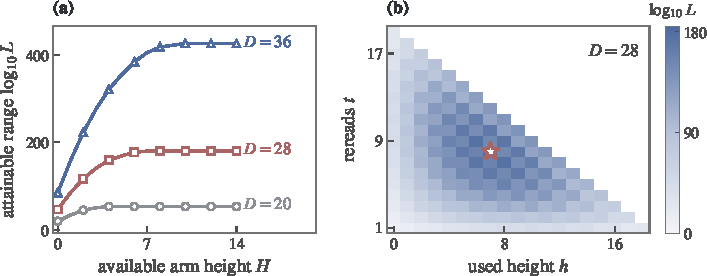
\includegraphics[width=5.2in]{FigS5.pdf}
\caption{\textbf{How much redundancy can a fixed duration use?}
(a) Achievable range versus available arm height $H$ at three fixed
budgets. Taller unused arms do not improve the construction once the
best allocation saturates. (b) At $D=28$, each point fixes used height
$h$ and resource rereads $t$, while optimizing block length and endpoint
reads. The star marks a maximum, and blank cells mark infeasible allocations. Both
panels assume ideal gates and storage, $p=1\%$, and operation error at most $5\%$.
Every quantum gate and readout layer is included.}
\label{fig:allocation}
\end{figure}


\paragraph*{Simultaneous endpoint and interface readout in Fig.~\ref{fig:reach}(b).}
Prepare the local Bell links as above. At each end, apply a CNOT
from the data qubit to the outer endpoint of its link, in the same layer
as the CNOTs of the interface Bell transformations. All these pairs
are disjoint. The following Hadamards act only at the interfaces.
The first and last blocks each have a free half-block for copying the
endpoint pointer. The endpoint and interface pointers can therefore
be copied in the same $\ell+h$ layers and measured in the same $t$
rounds. Each has $(\ell+1)(h+1)$ copies, including the original
pointer. Let $m$ be the largest odd integer at most $(\ell+1)(h+1)t$.
If one report must be omitted, its position is chosen before the run.

Condition on the true interface values and denote their correction
parities by $x,z$. The interface projections commute with the endpoint
CNOTs, so for true endpoint bits $u,v$ the data operator is proportional
to $Z_A^z P_{u\oplus v\oplus x}$, as in Sec.~\ref{sm:operations}.
Return $\hat u\oplus\hat v\oplus\hat x$ and apply $Z_A^{\hat z}$.
The final phase correction costs one local gate layer. The branch-operator
identity holds for every input, including data entangled with a reference.

For a block size $B=2\ell+2$, let $J=\lfloor(L+1)/B\rfloor$ be the number
of blocks and distribute the $r=L+1-BJ$ excess sites as evenly as
possible among them. Each half-block still fits, and moving the central
Bell pairs to their ends costs at most $\lceil r/(2J)\rceil$ additional
SWAP layers. Counting the Hadamard and CNOT that prepare each local link,
the two interface layers, and the final Pauli correction gives
\begin{equation}
 D_{\rm sched}=2\ell+h+t+5+\left\lceil\frac{r}{2J}\right\rceil .
 \label{eq:comb-fixed-distance-schedule}
\end{equation}
Each of the $J-1$ interfaces contributes one decoded bit to each
correction. The two endpoint decisions also enter the returned parity.
Their majority errors are independent, even when the true endpoint
values are correlated with the data, because the probability of a
majority error is the same for either true bit. With $a=1-2q_m(p)$,
Eq.~\eqref{eq:parity-exact-error} gives
\[
 \eps_{\rm op}=1-\frac{(1+a^{J-1})(1+a^{J+1})}{4}.
\]
At $L=8399$ and $p=0.10$, we minimize this error for each layer budget
$D$ over integer schedules with $D_{\rm sched}\le D$,
$\ell,t\ge1$, $0\le h\le H$, and $J\ge2$.

For the three schedules below, $J=2100$, $r=0$, and $\ell=1$. The
layouts have $33\,600$ resource sites and two endpoint data qubits each.
$H$ is the available arm height along the backbone, $h$ the height
used, and $Ct$ the number of acquired reports per pointer. All acquired
reports count toward the depth, including the one omitted when $Ct$ is even.
\begin{center}
\begin{tabular}{@{}lrrrrrrr@{}}
\toprule
Layout & $D$ & $H$ & $h$ & $t$ & $Ct$ & $m$ & $\eps_{\rm op}$\\
\midrule
Distributed & 12 & 3 & 2 & 3 & 18 & 17 & 0.046458\\
Distributed & 13 & 3 & 2 & 4 & 24 & 23 & 0.001961\\
Concentrated & 13 & 1 & 1 & 5 & 20 & 19 & 0.016303\\
\bottomrule
\end{tabular}
\end{center}
The concentrated schedule leaves the source reservoir idle. At $L=8399$,
disjoint backward cones exclude corrected Bell fidelity above $1/2$
for any measurement-free depth below 4200, even after endpoint-local
detection and classical processing.

One can isolate the effect of imperfect links in the same finite schedule.
Suppose each of the $J$ Bell links independently suffers a $Z$ fault on
one half after preparation, with probability $g$. All other quantum
operations are ideal and the binary reporting errors are as above. The fault changes the phase frame but leaves the Bell-outcome
probabilities unchanged. Its contribution to the final phase correction is
the parity of the $J$ faults, so the corrected $XX$ correlation acquires
the factor $(1-2g)^J$. In the simultaneous schedule the operation error is
then $1-(1+a^{J+1})[1+a^{J-1}(1-2g)^J]/4$, with $a=1-2q_m(p)$ as above.
For the 12-layer row, a phase-fault probability of $10^{-5}$ per prepared
link raises the error from $4.65\%$ to $6.56\%$.

\paragraph*{Using the phase-correction records in Fig.~\ref{fig:finite}(b).}
This comparison uses the resource-first schedule of
Eq.~\eqref{eq:comb-layer-schedule} and holds the quantum circuit and
every measurement fixed. Choose $\ell=h=2$, $t=3$, and $m_{\rm e}=5$, giving $D=20$,
$J=1400$ blocks at $L=8399$, and 27 acquired reports per Bell value.
At $p=0.10$, use all 27 reports for every bit correction, but only a
predetermined odd number $m_z\in\{1,3,\ldots,27\}$ for each phase
correction. Discard the remaining reports without conditioning on
their values. The two correction-error parities remain independent.
Set $\lambda_x=(1-2q_{27})^{1399}$,
$\lambda_z=(1-2q_{m_z})^{1399}$, and
$\zeta=(1-2q_5)^2$. The parity-result error $e_s$ and complete
instrument error are exactly
\begin{equation}
 e_s=\frac{1-\lambda_x\zeta}{2},\qquad
 \eps_{\rm op}=1-\frac{(1+\lambda_x\zeta)(1+\lambda_z)}4.
 \label{eq:partial-record-error}
\end{equation}
The parity-result error is input-independent. The corrected Bell input
attains the operation error by Eq.~\eqref{eq:parity-exact-error}. On this
fixed circuit $e_s=0.0170496$, while $\eps_{\rm op}$ falls from
$0.508525$ at $m_z=1$ to $0.0171270$ at $m_z=27$.

\subsection{The same qubit budget with different placements}
\label{sec:equal-budget}
For integer $H\ge1$, compare the uniform height-$H$ comb with a comb
whose arms all have height one except at the source. Extend the source
arm to height $1+(L+1)(H-1)$. Both graphs have exactly
$(L+1)(H+1)$ qubits, maximum degree three, backbone distance $L$,
and a unique path between the endpoints. A common source input qubit
may be added for transmission, or one common data qubit at each endpoint
for the parity operation.

For the concentrated layout and $d\ge1$, the source anchor contains
at most $6d+1$ cells. The disjoint cut neighborhoods chosen beyond it
contain at most $4d+2$ cells each, independently of the long arm's
height. The packing still gives $K\ge L/[8(d+1)]$.
Theorem~\ref{thm:range}, with $R\le bD$ and $d\le D$, therefore excludes
all endpoint entanglement unless $\ln L=O_{p,b}(D^2)$.
Ignoring the extra source qubits gives the matching deterministic
$\Theta(\sqrt{\ln L})$ construction. With uniform arms of height $H=\Theta((\ln L)^{1/3})$,
Eq.~\eqref{eq:comb-depth-optimal} gives the cubic exponent at the same
qubit count.

This lower bound does not require the concentrated resources to form
a long arm. Any ancillary graph of fixed maximum degree $\Delta$ attached
only at the source leaves the distant cut neighborhoods unchanged.
The source anchor has at most $\exp[O_\Delta(d)]$ cells. Its report budget
enters the right side of Eq.~\eqref{eq:cut-range}, whereas each distant
window contributes $\exp[-O_p(Rd)]$ to the left. Taking logarithms
again gives $\ln L=O_{p,b,\Delta}(D^2)$, independently of the total reservoir
size. Thus a compact planar reservoir at the source cannot replace
ancillas distributed along the path. All new graph connections must
remain confined to the source reservoir for this statement to apply.

\subsection{Narrow rectangular strips}
\label{sec:narrow-strips}
Consider the full rectangular nearest-neighbor graph with cells
$(x,y)$, $0\le x\le L$ and $0\le y<w$, at fixed local reporting
capacity $b$. Place the two data qubits at $(0,0)$ and $(L,0)$,
with product ancillas. For fixed $p,\eps$ and $C_0>0$, the optimal
duration of the complete parity instrument satisfies
\begin{equation}
 D^{\star}_{\eps,\mathrm{strip}}(L,w)
 =\Theta_{p,\eps,b,C_0}\!\left(\sqrt{\frac{\ln(L+1)}{w}}\right),
 \qquad 1\le w\le C_0[\ln(L+1)]^{1/3}.
 \label{eq:narrow-strip-time}
\end{equation}
The lower bound already holds for creating an entangled endpoint output
from product initialization in any positive-probability record.
Bell-pair distribution and transmission
have the same optimal order.

There are at most $bw(L+1)$ qubits, so the hardware bound in
Sec.~\ref{sec:square-unique-path} gives the lower bound even for one
entangled record. Alternatively, vertical cuts have radius-$d$
neighborhoods of at most $(2d+2)w$ cells, and the endpoint anchor
contains at most $(2d+1)w$. For the upper bound, use only horizontal
edges on the bottom row. This leaves a comb of height $H=w-1$, for
which Eq.~\eqref{eq:comb-depth-optimal} gives
$O_{p,\eps,b}(\max\{(\ln L)^{1/3},\sqrt{\ln L/w}\})$.
The width assumption makes the second term dominant up to a
$C_0$-dependent constant.

\subsection{Identical ancillary networks along a path}
\label{sec:reservoir-profile}

At every vertex of a backbone of length $L$, attach an identical rooted
ancillary graph, identifying only its root with that vertex. Different
attachments have no edges between them. Assume the entire graph has
maximum degree at most a fixed $\Delta$, with bounded local dimension
and reporting capacity as in the main text. Let $N(k)$ count cells in
one attachment within distance $k$ of its root, including the root.
The ancillary graph may depend on $L$. Define
\begin{equation}
 x_L=\min\{k\in\mathbb N:k\ge1,\ k^2N(k)\ge\ln(L+1)\}.
 \label{eq:reservoir-scale}
\end{equation}
At fixed $0<p<1/2$ and $0<\eps<1/2$, the optimal duration of the
complete remote parity instrument is
\begin{equation}
 D^\star_\eps(L)=\Theta_{p,\eps,b,\Delta}(x_L).
 \label{eq:reservoir-time}
\end{equation}
The lower bound already excludes arbitrarily weak endpoint entanglement
in any positive-probability record, starting from a state product across
cells. Constants are uniform over the ancillary graphs with this degree
bound, including graphs whose size and shape vary with $L$.

For a backbone cut, its radius-$d$ neighborhood contains at most
$v_d=2\sum_{r=0}^dN(r)$ cells. The radius-$2d$ region at the endpoint
contains at most $u_d=\sum_{r=0}^{2d}N(r)$ cells.
Cuts spaced by $2d+2$, excluding this region and the opposite endpoint,
supply $K\ge L/[8(d+1)]$ disjoint neighborhoods for
$L\ge16(d+1)$. Theorem~\ref{thm:range} gives separability whenever
\begin{equation}
 L\ge\max\left\{16(d+1),\,
 8(d+1)(\Lambda_pRu_d+\ln3)e^{\Lambda_pRv_d}\right\}.
 \label{eq:reservoir-strict}
\end{equation}
Bounded degree implies $\ln(u_D+1)=O_\Delta(D+1)$.
Using $d\le D$, $R\le bD$, and $v_D\le2(D+1)N(D)$, any entangled
branch must therefore satisfy
$\ln(L+1)\le C_{p,b,\Delta}D^2N(D)$.
This also holds for $L<16(D+1)$ after increasing the constant.
For $f(k)=k^2N(k)$, monotonicity gives
$f(k)\ge(k/D)^2f(D)$ when $k\ge D$.
Hence $x_L\le\lceil\sqrt{C_{p,b,\Delta}}D\rceil$, proving the
lower bound without an assumption of regular growth.

For achievability use the backbone blocks of
Sec.~\ref{sec:comb-construction} with $\ell=x_L$.
Copy each interface value into its assigned $\ell+1$ backbone vertices
and then into the radius-$\ell$ ball of each attached graph.
The groups are disjoint. A breadth-first spanning tree copies the
value through each ball in at most $\Delta\ell$ layers, scheduling
the outgoing edges of each parent separately.
Each interface value thus has $(\ell+1)N(\ell)$ identical pointers.
Keep an odd subset containing at least half of them and read each
$t$ times, with $t$ the least odd integer at least $C_{p,\eps}\ell$. Majority decoding bounds the total
resource error by
$2L\exp[-\kappa_p C_{p,\eps}\ell^2N(\ell)/2]\le\eps/2$
for a sufficiently large constant $C_{p,\eps}$.
The protected endpoint conversion in Sec.~\ref{sm:operations}
adds $O_{p,\eps}(1)$ layers and error at most $\eps/2$.
If fewer than two blocks fit, $L=O(\ell)$ and coherent Bell distribution
with the same endpoint conversion suffices.
The total duration is $O_{p,\eps,\Delta}(x_L)$.

Equation~\eqref{eq:reservoir-time} specifies the optimal duration.
For polynomial growth, it also gives the chain and comb reach laws
in the main text. For exponential growth, constant rescalings of time
change $N(D)$ exponentially, so one must retain them when discussing
reach. In particular, $N(D)=\Theta(2^D)$ gives $v_D=\Theta(2^D)$,
and Eq.~\eqref{eq:reservoir-strict} already bounds
$\ln L$ by $O_{p,b,\Delta}(D2^D)$. The general duration law does not imply
$\ln L=\Theta(D^2N(D))$ at a prescribed duration.

\subsection{Branching trees}
\label{sec:branching-tree}

Let $\Delta\ge3$ bound the degree of a tree and let the two outputs
have distance $L$. Cutting the unique path gives the packing estimate
above, with cut and anchor neighborhoods of sizes
\[
 |W_j|\le2\sum_{r=0}^d(\Delta-1)^r,\qquad
 |C|\le1+\Delta\sum_{r=0}^{2d-1}(\Delta-1)^r .
\]
With $d\le D$, $R\le bD$,
Eq.~\eqref{eq:cut-range} makes every reported endpoint
state separable beyond a distance
$\exp[\exp(O_{p,b,\Delta}(D))]$.
Hence every such tree requires
$D=\Omega_{p,b,\Delta}(\ln\ln L)$ for an entangled endpoint pair
or a non-entanglement-breaking transmission branch, at any yield.

This order is attainable on degree-three trees.
Prepare Bell pairs on disjoint backbone edges $(v_{2j},v_{2j+1})$
and apply Bell-basis transformations between successive pairs.
Join each measured backbone vertex by a single edge to the root of a
separate full binary tree of $N$ ancillas. Both the backbone vertex and
the new root have degree at most three. Copy the pointer value across
this edge and down the tree in $O(\ln N)$ layers, measure the ancillas
once, and majority decode.
With $N=O_{p,\eps}(\ln L)$, the total Bell-pair error is at most
$\eps$, while $D=O_{p,\eps}(\ln\ln L)$ and the number of qubits is
$O_{p,\eps}(L\ln L)$.
Local input injection with constant protected readout again gives
transmission in the same order.
Thus the optimal depth over bounded-degree trees for this two-endpoint
task is of order $\ln\ln L$.

\FloatBarrier
\section{The chain: finite-size bounds and optimal duration}
\label{sm:time}

For a chain, let
\begin{equation}
 s=2d+2,\qquad K=\left\lfloor\frac{L-1}{s}\right\rfloor,
 \qquad \xi=s e^{sR\Lambda_p}.
 \label{eq:range-scale}
\end{equation}
Setting $H=0$ in
Eq.~\eqref{eq:comb-reach} gives the transmission time
\begin{equation}
 \Dopt(L)=\Theta_{p,b,\eps}(\sqrt{\ln L})
 \label{eq:time}
\end{equation}
at fixed accuracy and readout error. The constructions
below exhibit the transition to coherent transport.

For a single qubit $A$ and all outputs $B$ at distance at least $L$
on either or both sides, we have
\begin{equation}
 L\ge4\xi\ln(2\xi)
 \quad\Longrightarrow\quad \rho_{AB|\boldsymbol y}\text{ is separable for every }\boldsymbol y.
 \label{eq:strict-main}
\end{equation}
To see this, replace all reports within distance $2d$ of $A$.
The resulting product contribution dominates $a\omega_{\boldsymbol y}$, where
$a=e^{-R(4d+1)\Lambda_p}$, and its $A$ factor is fixed under
conditioning outside this region. On each populated side choose
$K_\star=\lfloor(L-2d-1)/s\rfloor$ disjoint windows outside it.
A fully replaced window on each side isolates $A$ from all of $B$.
A union bound in CP order bounds the remaining relative weight by
$\Pi_\star=2(1-e^{-sR\Lambda_p})^{K_\star}$, including with the
anchor fixed. The separable-neighborhood proof in the End Matter
therefore applies whenever $\Pi_\star\le a/3$.
It suffices that $K_\star\ge e^{sR\Lambda_p}\ln(6/a)$.
Writing $x=sR\Lambda_p$ and rounding upward gives a sufficient
integer distance no larger than
$\xi(2e^{-x}+\ln6+2x)\le4\xi\ln(2\xi)$.
After tracing out the intervening registers, local filters and record
selection preserve separability.

For $p=0.4$, $d=1$ and $R=2$, Eq.~\eqref{eq:strict-main} gives $4\xi\ln(2\xi)=2182.829\ldots$, so $2183$ cells suffice for exact separability in every record. Figure~\ref{fig:finite}(a) gives exact thresholds for a specified circuit.

\begin{table}[tb]
\caption{\textbf{Optimal transmission time on a chain.} Entries denote $\Theta(\cdot)$ scalings at fixed width and Bell fidelity strictly between $1/2$ and one. The constructions use ideal quantum operations and fixed readout error $0<p<1/2$. The same noisy orders are necessary even to retain arbitrarily weak transmitted entanglement, at any positive postselection yield.}
\label{tab:times}
\centering
\renewcommand{\arraystretch}{1.15}
\begin{tabular}{@{}llc@{}}
\toprule
Readout & Protocol & $\Dopt$\\
\midrule
None & Unitary transport & $L$\\
Perfect & Teleportation & $1$\\
\addlinespace[3pt]
Noisy & One terminal round & $\ln L$\\
      & Fixed interaction depth & $\ln L$\\
      & Copies and rereads & $\bm{\sqrt{\ln L}}$\\
\bottomrule
\end{tabular}
\end{table}
The separating windows avoid the outputs throughout. Exact separability
also requires them to avoid the anchor.
Table~\ref{tab:times} summarizes the duration laws. The End Matter proves
Eq.~\eqref{eq:uniform-herald}, with
$s=2d+2$, $K=\lfloor(L-1)/s\rfloor$, and
$\Pi=(1-e^{-\Lambda_p Rs})^K$.
For $K\ge1$, accepted fidelity at least $1-\eps$ requires
\begin{equation}
 Rs\ln\frac{1-p}{p}
 \ge\ln K-\ln[-\ln(1-2\eps)].
 \label{eq:Snecessary}
\end{equation}
For $0<\eps\le\eps_0<1/2$, the last nested logarithm involves
$2\eps\le-\ln(1-2\eps)\le C_{\eps_0}\eps$,
where $C_{\eps_0}=-\ln(1-2\eps_0)/\eps_0$.
For $L\ge16$ and $1\le d\le L/16$,
$K\ge(L-1)/(4d)-1\ge L/(8d)$.
Consequently,
\begin{equation}
 R(2d+2)\Lambda_p
 \ge\ln\frac{L}{d\eps}-\ln(8C_{\eps_0}).
 \label{eq:tradeoff}
\end{equation}
The additive constant is independent of $p$.
If $d=0$, local operations and classical communication cannot transmit
entanglement. If $R=0$ and $d<L$, the output cannot depend on the input.

For total duration $D$, choose windows of length $2D+2$ and pad to $bD$
slots per cell. For $1\le D\le L/16$,
\begin{equation}
 bD(2D+2)\ln\frac{1-p}{p}+\ln D
 \ge\ln\frac L\eps-O_{\eps_0}(1).
 \label{eq:Sduration}
\end{equation}
At fixed $p,b$ its left side is $O(D^2)$. If $D>L/16$ the linear
alternative already holds. Small $L$ is absorbed into the constants.
Thus
$D=\Omega_{p,b,\eps_0}(\min\{L,\sqrt{\ln[(L+1)/\eps]}\})$,
independently of the acceptance probability. A deterministic protocol with
half-diamond error at most $\eps$ also has Bell fidelity at least
$1-\eps$, so the converse applies to that stronger error criterion.
The construction in Sec.~\ref{sm:wire-upper} supplies the matching
upper bounds.

With one terminal readout round, a fixed local circuit is followed by
simultaneous measurement and a product correction channel. Bounded width
gives $R=O(1)$, so Eq.~\eqref{eq:Snecessary} yields
$D=\Omega_p(\min\{L,\ln[(L+1)/\eps]\})$.
For fixed $d\ge1$, $L\ge16d$, and $0<\eps\le\eps_0<1/2$,
Eq.~\eqref{eq:tradeoff} gives
$R=\Omega_{p,d,\eps_0}(\ln[(L+1)/\eps])$.
The repeated-readout ladder below attains the latter bound in
$D=O_p(\ln[(L+1)/\eps])$.

\paragraph*{Unconditional channel and exact transmission.}
Before conditioning on success, each fully replaced window has
probability $(2p)^{Rs}$. Set
\begin{equation}
 \Pi_{\rm av}=\bigl[1-(2p)^{Rs}\bigr]^K,\qquad
 \channel=(1-\Pi_{\rm av})\channel_{\EB}+\Pi_{\rm av}\channel_* .
 \label{eq:unconditional}
\end{equation}
At least one uninformative window occurs with input-independent
probability $1-\Pi_{\rm av}$. Conditioned on this event, the channel is
entanglement breaking by cut deletion. The same statement holds with the complete
record at the receiver, since the Choi operator in each fixed branch is
separable. Consequently
$\Fe\le(1+\Pi_{\rm av})/2$ and
$d_\diamond(\channel,\channel_{\EB})\le \Pi_{\rm av}$.
For the binary detector, $\Pi_{\rm av}\le\Pi$.
The unconditional bound uses $\ln[1/(2p)]$ in place of
$\ln[(1-p)/p]$ in Eq.~\eqref{eq:Snecessary}.

Exact accepted transmission requires $d\ge L$ for any $p>0$ and a finite
number of reports. For a fixed record $\boldsymbol y$ containing $n_{\boldsymbol y}$ reports,
let $\mathcal T_{\boldsymbol y}$ be the trace-preserving frozen-controller circuit with
all measurements made nonselective. Positivity of the instrument maps gives
$p^{n_{\boldsymbol y}}\mathcal T_{\boldsymbol y}\preceq_{\rm CP}\channel_{\boldsymbol y}
\preceq_{\rm CP}(1-p)^{n_{\boldsymbol y}}\mathcal T_{\boldsymbol y}$.
For $d<L$ the output of $\mathcal T_{\boldsymbol y}$ is independent of the input,
and its Choi state is product.
Any receiver filter accepting the $\boldsymbol y$ branch with positive probability
therefore accepts a positive product contribution from $\mathcal T_{\boldsymbol y}$.
The accepted Choi state cannot be a pure Bell state.

\paragraph*{Uniform readout dependence at fixed accuracy.}
Fix $0<\eps<1/2$. For $\alpha>0$, let
$x_\alpha$ be the unique positive solution of
\begin{equation}
 \alpha x_\alpha^2=\ln(L/x_\alpha).
 \label{eq:information-scale}
\end{equation}
For a fixed strip supporting the construction,
\begin{equation}
 D_{\eps,\bullet}^{\star}(L,p)
 =\Theta_{b,\eps}\!\left(\min\{L,\max\{1,x_\alpha\}\}\right),
 \quad
 \alpha=
 \begin{cases}
 \kappa_p,&\bullet=\mathrm{det},\\
 \Lambda_p,&\bullet=\mathrm{her}.
 \end{cases}
 \label{eq:uniform-information-time}
\end{equation}
The constants are independent of $p,L$. We test the reference--output Bell fidelity, allowing selection at any positive yield. The deterministic construction also controls half-diamond error.
For $K\ge1$, the exact branch bound $n\Lambda_p\ge-\ln(2\eps)>0$ absorbs the additive constant in Eq.~\eqref{eq:tradeoff}.

For the deterministic lower bound, set $\delta=1-2\eps$.
When $1\le D\le L/16$, $n=R(2d+2)\le4bD^2$ and
$K\ge L/(8D)$ give
$8b\kappa_pD^2\ge\ln[1+\delta^2L/(8D)]$.
If $x_{\kappa_p}\ge1$ and
$D\le c x_{\kappa_p}$, choose
$c\le\min\{1/32,\delta^2/8,1/(4\sqrt b)\}$.
The right side is then at least $\ln(L/x_{\kappa_p})$,
while the left side is at most half that value, a contradiction.
For $x_{\kappa_p}<1$ one nontrivial layer supplies the lower bound.
For heralding the same comparison uses Eq.~\eqref{eq:Snecessary} and a smaller $c=c_{b,\eps}$.

For achievability take $\ell=t$ to be the next odd integer at least
$C_\eps\max\{1,x_\alpha\}$, with
$C_\eps\ge3$ and
$C_\eps^2\ge1+\ln(2/\eps)/\ln2$.
If $\ell\le L/2$, then
$\alpha\ell^2\ge\ln[2L/(\ell\eps)]$, and the protected wire
has error at most $\eps$. Use majority decoding for
$\alpha=\kappa_p$ and unanimous-report selection for
$\alpha=\Lambda_p$. If $\ell>L/2$, exact SWAP transmission takes
$L<2\ell$ layers and preserves the same order bound.
Equation~\eqref{eq:unanimity-uniform} extends the heralded result uniformly to all $0<\eps\le\eps_0<1/2$.
Ideal teleportation has constant depth at $p=0$. At $p=1/2$ the
reports contain no information and linear interaction depth is necessary.

\paragraph*{Separated output regions.}
Let $A$ and $B$ be fixed output regions on opposite sides of an interval
of $r-1$ cells. Start from a state product across cells and discard all
quantum registers outside these regions after the costed protocol.
For every reported branch, and after any positive-probability classical
selection and local filters on $A$ and $B$,
\begin{equation}
 \inf_{\sigma\in\operatorname{Sep}(A:B)}
 \frac12\|\rho_{AB}^{\rm acc}-\sigma\|_1
 \le
 \left[1-e^{-\Lambda_p R(2d+2)}\right]^{{\lfloor
 (r-1)/(2d+2)\rfloor}}.
 \label{eq:separated-regions}
\end{equation}
Place the windows inside the gap and apply Eq.~\eqref{eq:uniform-herald}
to their cut decomposition. A classical copy of the record can be
retained on either or both sides. Quantum operations on the intervening
registers are included in the protocol depth.

\paragraph*{A bounded region and all distant outputs.}
The strict theorem extends to any fixed output region. Let $A$ be
contained in an interval of $r$ cells,
and let $B$ lie outside the $L$-neighborhood of that enclosing interval,
on either or both sides.
Replace all reports within distance $2d$ of the enclosing interval of
$A$. The product contribution dominates
$a_A\omega_{\boldsymbol y}$, with $a_A=e^{-\Lambda_p R(r+4d)}$, and its $A$ factor
remains fixed under outside-flag conditioning. A replaced window on each populated side isolates $A$, leaving
residual relative weight at most $\pi=2(1-e^{-\Lambda_p Rs})^{\lfloor(L-2d-1)/s\rfloor}$.
Using Lemma~\ref{lem:one-sided-separable} on the support of the product contribution, the proof of Theorem~\ref{thm:range} applies whenever
$\pi\le a_A/(\dim A+1)$. Thus a sufficient distance is
\begin{equation}
 L\ge 2d+1+s\left\lceil e^{sR\Lambda_p}
 \left[\ln(2(\dim A+1))+R(r+4d)\Lambda_p\right]\right\rceil.
 \label{eq:bounded-region-range}
\end{equation}
For fixed $r$ and $\dim A$, this is $O_{r,\dim A}(\xi\ln(2\xi))$.
All intervening registers are traced out after the costed protocol.
This statement does not require, or imply, separability of two
unrestricted half-chains or of the entire prepared state.

\paragraph*{Reporting capacity and width.}
If each cell contains $w$ qubits and the protocol uses $t$ readout layers,
with at most one report per qubit per layer, then $R\le wt$.
Equation~\eqref{eq:tradeoff} implies
\begin{equation}
 wt(2d+2)\Lambda_p
 \ge\ln\frac{L}{d\eps}-O_{\eps_0}(1),
 \qquad 1\le d\le L/16.
 \label{eq:width-budget}
\end{equation}
In particular, fixed $d,t$ require $w=\Omega_p(\ln L)$ at fixed
accuracy. This is a necessary condition. A transverse copying chain
on a rectangular nearest-neighbor strip takes time proportional to its
height, so this substitution alone does not give a matching
constant-duration construction as width grows. For a full rectangular
nearest-neighbor strip, Eq.~\eqref{eq:narrow-strip-time} gives matching
bounds when $w=O((\ln L)^{1/3})$. For circuit noise in a fault-tolerant quantum bus, Choe and
K\"onig give an $O(\ln^2 L)$ construction and an $\Omega(\ln L)$ lower
bound on qubits per station~\cite{Choe2024}. On a planar strip of polylogarithmic width, Corollary~8.2.2 of
Ref.~\cite{Harley2026} gives a constant-depth resource whose bulk is
measured in $Z$, followed by a Pauli correction on a retained qubit.
With ideal gates and storage, read each measured bulk qubit an odd
number of times and take the majority. The decoded flips have
independent probability $q_t(p)$. The joint state of the decoded record and
the surviving qubits is the same as for independent $X$ faults on
the measured bulk qubits immediately before ideal $Z$ measurement.
For fixed $p<1/2$ and fixed target Bell fidelity, a constant number of
rounds puts $q_t(p)$ below the threshold of the corollary. The conversion
in Sec.~\ref{sm:operations} gives a complete parity measurement with
constant additional depth at fixed accuracy. Whether logarithmic width
suffices remains open.

For several classes of prescribed noisy channels, homogeneous repeater chains
with intermediate LOCC likewise require logarithmically many parallel uses per
link to retain a nonvanishing amount of entanglement~\cite{Masajada2026}.
Here the noisy elements are the reports generated during the circuit.

\paragraph*{Different gate and measurement times.}
Suppose a gate layer takes time $\tau_g>0$ and a readout round takes time $\tau_m>0$, with fixed reporting error $p$ per round. For a fixed-width strip supporting the construction, the optimum physical duration satisfies
\begin{equation}
 \Topt(L)=
 \Theta_{p,b,\eps_0}\!\left(
 \min\left\{\tau_gL,\,
 \tau_g+\tau_m+\sqrt{\tau_g\tau_m\ln\frac{L+1}{\eps}}\right\}\right).
 \label{eq:weighted-time}
\end{equation}
For the upper bound, choose odd integers of the orders
\[
 \begin{aligned}
 \ell&=\max\left\{3,\sqrt{\frac{\tau_m}{\kappa_p\tau_g}
                         \ln\frac{L+1}{\eps}}\right\},\\
 t&=\max\left\{1,\sqrt{\frac{\tau_g}{\kappa_p\tau_m}
                         \ln\frac{L+1}{\eps}}\right\},
 \end{aligned}
\]
rounded upward with a sufficiently large constant multiplier. Then $\ell t$ supplies the required logarithmic redundancy, while the cost is $O(\tau_g\ell+\tau_mt)$. Taking the faster of this schedule and coherent SWAP transmission gives the minimum in the bound. If the construction requires $\ell$ comparable to $L$, its predicted cost is already of order $\tau_gL$, so the SWAP fallback preserves Eq.~\eqref{eq:weighted-time}.

For the lower bound, $d\le T/\tau_g$ and $R\le bT/\tau_m$. If the interaction depth is a fixed fraction of $L$, or if no reports are used, coherent causality gives the first alternative. Otherwise Eq.~\eqref{eq:tradeoff} applies. A successful protocol in this regime uses both an interaction and a report, so $T\ge\max\{\tau_g,\tau_m\}$. In particular,
$\ln d\le d\le T/\tau_g\le T^2/(\tau_g\tau_m)$.
Combining $T^2/(\tau_g\tau_m)=\Omega_{p,b,\eps_0}(\ln[(L+1)/\eps])$ with the minimum layer times proves the second alternative. The bound assumes a fixed error per readout round. Changing a detector's integration time may also change $p$ and is a separate optimization.

For the two finite schedules used in Fig.~\ref{fig:reach}(b), the first
depths reaching $5\%$ error take $9\tau_g+3\tau_m$ (distributed) and
$8\tau_g+5\tau_m$ (concentrated). At 13 layers their respective
schedule families achieve $0.20\%$ and $1.63\%$ error. Counting each
SWAP as three CNOTs instead of one gate changes the explicit 12-layer
schedule to 14 layers, compared with the same coherent lower bound
of 4200 layers.

\paragraph*{Unequal operation times on a comb.}
The height-dependent law also extends to physical time. Assume
nondemolition readout is available, with layer costs $\tau_g,\tau_m>0$
and fixed reporting error $0<p<1/2$. Fix $0<\eps<1/2$ and the local
reporting capacity $b$, and write $S=\ln(L+1)$. Then
\begin{equation}
 \Topt(L,H)=
 \Theta_{p,\eps,b}\!\left(
 \min\left\{\tau_gL,\,
 \tau_g+\tau_m+
 \max\left\{(\tau_g^2\tau_m S)^{1/3},
              \sqrt{\frac{\tau_g\tau_m S}{H+1}}\right\}\right\}
 \right).
 \label{eq:weighted-comb-time}
\end{equation}
The constants are independent of $H,\tau_g,\tau_m$. The lower
bound applies to a single entangled transmission branch, and a
deterministic protocol attains the stated accuracy.

For the lower bound, a protocol of duration $T$ has
$d\le T/\tau_g$ and $R\le bT/\tau_m$.
If $T\ge\tau_gL/32$, the first alternative already supplies the bound.
Otherwise successful transmission requires an interaction and a
report, so $d,R\ge1$ and $T\ge\max\{\tau_g,\tau_m\}$.
The packing condition in Eq.~\eqref{eq:comb-exact-separability}
then holds. Its sufficient separability condition must fail for an
entangled output. Using
$u_d(H),v_d(H)=O[d\min\{d,H+1\}]$ gives
\[
 S\le C_p R d\min\{d,H+1\}.
\]
The logarithms of the packing prefactor and anchor weight are
absorbed because $R d\min\{d,H+1\}\ge d\ge1$.
Substituting the time budgets proves both
$T^3\gtrsim_{p,b}\tau_g^2\tau_m S$ and
$T^2\gtrsim_{p,b}\tau_g\tau_m S/(H+1)$.
Together with the minimum layer times, these give the lower bound.
Bounded $L$ changes only constants.

For achievability, set
\[
 x=\max\left\{1,\left(\frac{\tau_m S}{\tau_g}\right)^{1/3},
                  \sqrt{\frac{\tau_m S}{\tau_g(H+1)}}\right\}.
\]
Choose $\ell=\lceil Cx\rceil$ and take $t$ to be the next odd integer
above $C\max\{1,S/[x\min\{x,H+1\}]\}$.
A sufficiently large $C=C_{p,\eps}$ makes the existing comb
construction accurate enough. Since
$x^2\min\{x,H+1\}\ge(\tau_m/\tau_g)S$,
its cost is $O_{p,\eps}(\tau_gx+\tau_m)$, including rounding
and protected input injection. If the intervals do not fit,
$L<8\ell$, SWAP transmission costs $O(\tau_gL)=O_{p,\eps}(\tau_gx)$.
Otherwise choose the faster of the protected construction and SWAP
transmission. This proves Eq.~\eqref{eq:weighted-comb-time}.

When neither minimum layer costs nor coherent transport dominate,
the long-arm regime begins at
$H+1\gtrsim_{p,\eps}[(\tau_m/\tau_g)\ln(L+1)]^{1/3}$.
For fixed layer times, the corresponding large-distance time scales
are $(\tau_g\tau_m\ln L)^{1/2}$ on the chain and
$(\tau_g^2\tau_m\ln L)^{1/3}$ on the long-arm comb. Fresh-probe readout gives a corresponding upper bound
when its copying and reset costs are included in the time per round.

\paragraph*{Physical duration of the parity operation.}
At fixed $p$, $\eps<1/2$, and local capacity, the nondestructive parity
measurement has optimum
\begin{equation}
 \begin{split}
 T_{\eps,ZZ}^{\star}(L,H)=\Theta_{p,\eps,b}\!\Bigg(
 \tau_m+\min\Bigg\{\tau_gL,\ \tau_g+
 \max\bigg\{&[\tau_g^2\tau_m\ln(L+1)]^{1/3},\\[-2pt]
 &\sqrt{\frac{\tau_g\tau_m\ln(L+1)}{H+1}}\bigg\}\Bigg\}\Bigg).
 \end{split}
 \label{eq:weighted-parity-time}
\end{equation}
The constants are uniform in positive $\tau_g,\tau_m$ and integer $H\ge0$.
The returned bit is an actual output of the classical controller,
computed from its reports and independent randomness. If there are no
reports, its distribution is independent of the data input. Comparing
one even-parity and one odd-parity $Z$ eigenstate then gives worst-case
half-diamond error at least $1/2$. Hence a successful implementation
must have duration at least $\tau_m$.

The parity-to-Bell test in Sec.~\ref{sm:operations} also gives the
Bell-generation lower bound used in Eq.~\eqref{eq:weighted-comb-time}.
The final record-dependent correction is local and introduces neither
a new report nor spreading of quantum support, so the same resource
count applies to the test. Combining that bound with $T\ge\tau_m$
proves the lower bound in Eq.~\eqref{eq:weighted-parity-time}.

For the upper bound, the protected Bell construction and the two
protected endpoint readouts cost
$O_{p,\eps,b}(\tau_g+\tau_m)$ plus the maximum term in
Eq.~\eqref{eq:weighted-parity-time}. Alternatively, a traveling ancilla
accumulates parity by a CNOT from the first data qubit, SWAPs along the
backbone, and a CNOT from the second data qubit. Reading this pointer
with $O_{p,\eps}(1)$ repeated reports implements the parity instrument
in $O_{p,\eps}(\tau_g L+\tau_m)$ time. Taking the faster construction
proves the stated optimum. The final readout cost distinguishes this
operation from measurement-free coherent transmission.

\FloatBarrier
\section{Quantum transmission with spatial copies and repeated readout}
\label{sm:wire-upper}

\paragraph*{Block layout and Bell links.}
Choose odd integers $\ell\geq3$ and $t\geq1$. If $L<2\ell$, use
successive SWAP gates along the main row to transmit the input exactly
in duration $O(L)$, with no measurements. Otherwise let
$M=\lfloor L/\ell\rfloor$. Partition cells $1,\ldots,L$ into $M$
consecutive blocks of length $\ell$, adding the remaining
$L-M\ell$ sites to the last block. Every block therefore has room
for $\ell$ spatial copies. Denote the left and right main-row endpoints
of block $j$ by $A_j$ and $B_j$.

In parallel in all blocks, prepare
$\lvert\Phi^+\rangle_{A_jB_j}$ by creating a Bell pair on the first
two sites and moving its second half to $B_j$ by adjacent SWAPs.
This takes $O(\ell)$ nearest-neighbor layers, including a constant
factor if each SWAP is decomposed into CNOTs. All block interiors
return to $\lvert0\rangle$. No copy or measurement is used to create
these links.

Let $A_{\rm in}$ be the input at cell $0$. Apply the Bell-basis transformations
\begin{equation}
 \mathrm{CNOT}_{A_{\rm in}\to A_1},\ H_{A_{\rm in}};
 \qquad
 \mathrm{CNOT}_{B_j\to A_{j+1}},\ H_{B_j}
 \quad(1\leq j<M).
 \label{eq:wire-bell-transform}
\end{equation}
These disjoint transformations measure $2M$ Bell bits, including the
two injection bits. The output $B_M$ is kept.

\paragraph*{Explicit copying paths on four rows.}
Each cell is a column of four qubits in rows $0,1,2,3$.
The links and input occupy row $0$.
Only rows $1,2$ are needed away from the first block. Protect each
Bell-measurement qubit with exactly $\ell$ distinct ancillary copies, as follows.
\begin{enumerate}
\item Copy $A_{\rm in}$ into row $3$ at cell $0$ through the two initially
zero intermediate qubits at that cell. Writing these as $a,b,c$ in
rows $1,2,3$, use
\[
 \mathrm{CNOT}_{A_{\rm in}\to a},\quad
 \mathrm{CNOT}_{a\to b},\quad
 \mathrm{CNOT}_{b\to c},\quad
 \mathrm{CNOT}_{a\to b},\quad
 \mathrm{CNOT}_{A_{\rm in}\to a}.
\]
This leaves only $c$ carrying the copied computational-basis value
and restores $a,b$ to zero. Propagate $c$ rightward along row $3$
through cells $0,\ldots,\ell-1$.
\item For each measured right endpoint $B_j$, $j<M$, first copy
vertically to row $2$. Using the initially zero intermediate row-$1$
qubit $a$ and row-$2$ qubit $b$ at the same cell, apply
$\mathrm{CNOT}_{B_j\to a}$,
$\mathrm{CNOT}_{a\to b}$,
$\mathrm{CNOT}_{B_j\to a}$.
Then propagate leftward through the last $\ell$ cells of its own
block along row $2$.
\item Copy each $A_j$, $1\leq j\leq M$, vertically to row $1$
and then rightward through the first $\ell$ cells of its own block.
\end{enumerate}
Perform the vertical operations in this order, then propagate along
all three rows in parallel. The paths are disjoint within each row, so
copying takes $O(\ell)$ layers. Each path implements
$\ket{s}\ket{0^\ell}\mapsto\ket{s}\ket{s^\ell}$ on a qubit to be
measured in $Z$. Measuring the copies implements that projection and
the original pointer can be discarded without readout.

\paragraph*{Stable pointers and fresh probes.}
Destructive detection is also possible with a stable pointer $C$.
Couple it by $\mathrm{CNOT}_{C\to A}$ to an adjacent probe in
$\ket0$, measure the probe in $Z$, and reset it. The pointer instrument
is $\rho\mapsto P_s\rho P_s$ with $P_s=\ket{s}\bra{s}$, including for
an entangled initial pointer. Later rounds read the same value.
All pairs operate in parallel, adding one probe per pointer and one
copying, measurement, and reset layer per round. With ideal pointer
storage, copying, and reset this preserves $D=O(\ell+t)$ and gives
$\ell t$ independent reporting errors per Bell bit.

\paragraph*{Repeated readout and channel error.}
With nondemolition readout, measure each spatial copy $t$ times in $Z$.
Since $P_s^t=P_s$, the extra observations leave the same projection on
the data. The majority of the odd number $\ell t$ of reports errs with
probability
\begin{equation}
 q=q_{\ell t}(p):=
 \Pr\{\operatorname{Bin}(\ell t,p)>\ell t/2\}
 \leq e^{-\kappa_p\ell t},
 \qquad \kappa_p=-\ln(2\sqrt{p(1-p)}).
 \label{eq:wire-majority}
\end{equation}
The decision-error variables are independent across measured qubits and
independent of their true values, including when conditioned on the
entire ideal quantum measurement record.

Label the Bell outcomes at interface $j=0,\ldots,M-1$ by
$(z_j,x_j)$, with $z_j$ the transformed control outcome and $x_j$
the transformed target outcome in Eq.~\eqref{eq:wire-bell-transform}.
The standard teleportation identity, iterated through the links,
gives the unnormalized branch operator from $A_{\rm in}$ to $B_M$ as
\begin{equation}
 K_s=2^{-M}e^{i\theta_s}
 X^{\bigoplus_jx_j}Z^{\bigoplus_jz_j}.
 \label{eq:wire-kraus}
\end{equation}
This holds on any reference-entangled input. After correction using the
decoded bits, the remaining Pauli exponents are parities of their
independent majority errors $E_{x,j},E_{z,j}$, giving
\begin{equation}
 \mathcal N(\tau)=
 \mathbb E\!\left[X^{E_X}Z^{E_Z}\tau Z^{E_Z}X^{E_X}\right],
 \qquad
 E_X=\bigoplus_{j=0}^{M-1}E_{x,j},\quad
 E_Z=\bigoplus_{j=0}^{M-1}E_{z,j}.
 \label{eq:wire-pauli-channel}
\end{equation}
The two parities $E_X,E_Z$ are independent, and each equals zero with
probability $[1+(1-2q)^M]/2$. Thus the entanglement fidelity and half-diamond
error are
\begin{align}
 \Fe(\mathcal N)&=
 \left[\frac{1+(1-2q)^M}{2}\right]^2,
 \label{eq:wire-fidelity}\\
 d_\diamond(\mathcal N,\id)
 &=1-\Fe(\mathcal N)\leq2Mq
 \leq\frac{2L}{\ell}e^{-\kappa_p\ell t}.
 \label{eq:wire-exact-error}
\end{align}
A Bell input distinguishes the four Paulis, attaining the triangle
inequality bound on the diamond distance. For $L=10^6$, $\ell=t=3$
give $M=333\,333$ and a final block of four cells. At $p=0.01$,
$q=1.218536857\times10^{-8}$ and $\Fe=0.9919257007$.

\paragraph*{Resources and matching range.}
For the layout in Fig.~\ref{fig:Swire}, the interaction depth is
$d=O(\ell)$, the total number of raw reports
at one longitudinal cell is at most $R=3t$, and the duration is
$D=O(\ell+t)$. Only the injection region needs three copies at one cell. Bulk cells
have at most two, so their report budget is $2t$. There are
$2M\ell$ measured ancillas, each read $t$ times, and no other reported
outcomes. Taking $\ell,t$ to be the next odd integers above
\[
 \max\!\left\{3,
 \sqrt{\kappa_p^{-1}\ln\frac{2(L+1)}{\eps}}\right\}
\]
proves the upper bound in Eq.~\eqref{eq:time}, using the SWAP fallback whenever
$L<2\ell$.

For Bell-pair distribution without an input, omit injection and keep
$A_1,B_M$ as outputs. A final nearest-neighbor SWAP moves $A_1$ from cell $1$ to the unused qubit at cell $0$ when that endpoint is prescribed. This costs constant time. Only rows $0,1,2$ are needed, and the exact
formula in Eq.~\eqref{eq:wire-fidelity} has $M-1$ in place of $M$.
\begin{figure}[t]
\centering
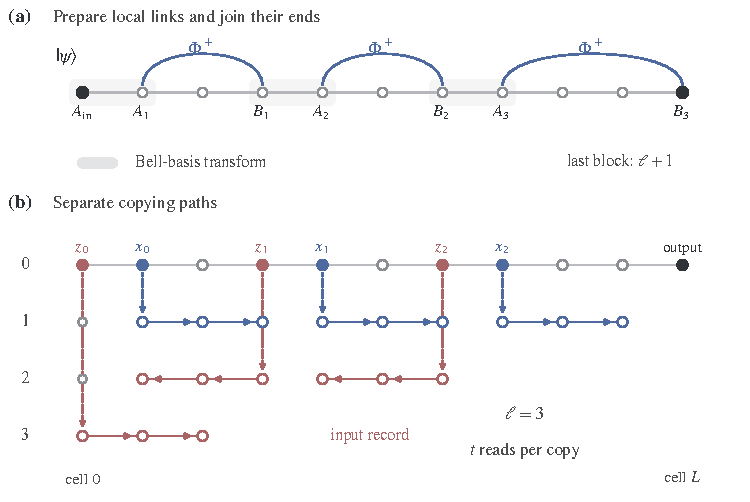
\includegraphics[width=5.0in]{FigS1.pdf}
\caption{\textbf{Four-row transmission with disjoint copying paths.}
(a) Local Bell links (arcs) and Bell-basis transformations (shaded pairs).
(b) Copying layout for $\ell=3$ and $L=10$. Blue paths carry $x$
values and red paths carry $z$ values, with row 3 reserved for $z_0$.
Dashed vertical transfers precede horizontal copying and restore borrowed
intermediate qubits to zero. Each copy is read $t$ times. Unused ancillary sites are omitted. The final block has four cells,
leaving enough space for every copy without measuring the output.}
\label{fig:Swire}
\end{figure}

\paragraph*{Constant interaction depth with repeated readout.}
A two-row nearest-neighbor strip realizes the constant-depth endpoint of
the tradeoff. Label the two qubits in cell $i$ by $a_i,b_i$, with their
upper and lower row assignments exchanged on alternating cells. Then
$a_i$ and $b_{i+1}$ are horizontal nearest neighbors, and all pairs
$(a_i,b_{i+1})$, $0\le i<L$, are disjoint. Prepare a Bell pair on each of
these pairs in parallel. Put the unknown input in $b_0$ and apply the
Bell-basis transformation to $(b_i,a_i)$ within each cell
$0\le i<L$. Read each of these $2L$ qubits in $Z$ for an odd number $t$
of rounds, majority-decode each bit, and apply the corresponding Pauli
correction to $b_L$. All premeasurement operations have constant depth
using horizontal and vertical edges of the rectangular graph.
If $q_t(p)$ is the majority error for $t$ independent binary reports, the
exact channel is the same Pauli channel as in the block construction,
with $M=L$ and $q=q_t(p)$. Hence
$1-\Fe\le2Lq_t(p)\le2L\exp(-\kappa_p t)$, also bounding the
half-diamond error. The largest number of reports at a cell is $2t$ and
the duration is $t+O(1)$. Choosing
$t=O_p(\ln[(L+1)/\eps])$ therefore attains the logarithmic readout
requirement at constant interaction depth without spatial copying.

\FloatBarrier
\section{Unanimous reports and the noise dependence of heralded transmission}
\label{sm:unanimity}

The transmission circuit has $M$ Bell measurements, including input
injection. To select a run, accept each Bell bit only when all its
$m=\ell t$ reports agree, and accept the run only when every Bell bit
passes. This rule and majority decoding have been tested with repeated
mid-circuit measurements~\cite{Koh2026} and with ancilla-encoded
readout~\cite{Czaban2026}. For either true value of one bit,
\begin{equation}
 a_m=(1-p)^m+p^m,\qquad
 q_m=\frac{p^m}{a_m}
     =\frac{1}{1+e^{m\Lambda_p}},
 \label{eq:unanimity-bit}
\end{equation}
where $a_m$ is its acceptance probability and $q_m$ its conditional
decoding error. Unlike majority decoding, this rule does not require
$m$ to be odd.

Both $a_m$ and $q_m$ are independent of the true bit. Global acceptance
therefore leaves the Bell transcript uniform, with independent residual
errors of probability $q_m$. Substitution in
Eqs.~\eqref{eq:wire-pauli-channel}--\eqref{eq:wire-exact-error} gives an
input-independent yield and a normalized Pauli channel,
\begin{equation}
 \begin{aligned}
 a&=a_m^{2M},\\
 \Fe^{\rm acc}
  &=\left[\frac{1+(1-2q_m)^M}{2}\right]^2
    =\left[\frac{1+\tanh(m\Lambda_p/2)^M}{2}\right]^2,\\
 d_\diamond(\channel_{\rm acc},\id)
  &=1-\Fe^{\rm acc}
    \le 2M e^{-m\Lambda_p}.
 \end{aligned}
 \label{eq:unanimity-channel}
\end{equation}
Thus $\Lambda_p\ell t\ge\ln[2L/(\ell\eps)]$ suffices for error $\eps$
on the stated block layout, with $d=O(\ell)$, $R\le3t$, and $D=O(\ell+t)$.

\paragraph*{Average output and the best complete record.}
The wire also distinguishes loss of entanglement in the averaged output
from loss in every reported branch. The ideal Bell bits are jointly uniform
and independent of the input, by Eq.~\eqref{eq:wire-kraus}. For a complete
record containing $k$ ones among $m$ reports of one bit, its optimal
posterior error is $[1+\exp(\Lambda_p|m-2k|)]^{-1}$. Hence every bit has
posterior error at least
$q_m=[1+\exp(m\Lambda_p)]^{-1}$, with equality for unanimous reports.
The posterior errors remain independent across Bell bits. After the
optimal Pauli correction, the largest Bell eigenvalue is maximized by
making each bit unanimous, giving the fidelity in
Eq.~\eqref{eq:unanimity-channel}. A two-qubit Bell-diagonal state is
separable if and only if its largest eigenvalue is at most $1/2$.
Consequently, the first number of interfaces for which all complete
records of this wire are entanglement breaking is
\begin{equation}
 M_{\rm EB}^{\rm all}
 =\left\lceil
 \frac{\ln(\sqrt{2}-1)}{\ln(1-2q_m)}
 \right\rceil.
 \label{eq:wire-all-record-range}
\end{equation}
The same expression with the majority error $q$ from Eq.~\eqref{eq:wire-majority}
gives the threshold for the majority-corrected channel after averaging
the detailed reports. At $p=0.01$ and $m=3$, the averaged wire first
becomes entanglement breaking at $M=1479$. A unanimous record still
leaves an entangled pair up to $M=427597$. From $M=427598$ onward,
every record is separable even after endpoint-local filtering.
At $M=427597$, accepting every string of unanimous triples gives log yield
$2M\ln[(1-p)^3+p^3]\simeq-25784$. One specified string has probability
$\{[(1-p)^3+p^3]/2\}^{2M}$. All these strings yield the same corrected Bell fidelity.
Figure~\ref{fig:finite}(a) converts the largest Bell weight of each
state to concurrence. The probabilities quoted in its caption include
all records that leave the endpoints entangled. With three reports,
a group splits two votes to one with probability $3p(1-p)$, in which
case its posterior bit error is $p$. For either Pauli correction the
number $i$ of split groups is thus binomial with parameters $M$ and
$3p(1-p)$. Its conditional parity bias is
$v_i=(1-2p)^i(1-2q_3)^{M-i}$, where $q_3$ is the unanimous error
in Eq.~\eqref{eq:unanimity-bit}. For independent split counts $i,j$
in the two corrections, the largest Bell weight is
$(1+v_i)(1+v_j)/4$. Summing their binomial probabilities wherever
this weight exceeds $1/2$ gives the entangled-record probability.

\begin{corollary}[Uniform reporting-error dependence]
On the fixed strip supporting this construction, let
$D_{\eps,\mathrm{her}}^{\star}(L,p)$ be the minimum duration for accepted
Bell fidelity at least $1-\eps$ at any positive yield.
For $0<p<1/2$, $0<\eps\le\eps_0<1/2$, and integer $L\ge1$, let
$x>0$ be the unique solution of
\begin{equation}
 \Lambda_p x^2=\ln\frac{L}{\eps x},
 \qquad
 D_{\eps,\mathrm{her}}^{\star}(L,p)
   =\Theta_{b,\eps_0}\!\left(\min\{L,\max\{1,x\}\}\right).
 \label{eq:unanimity-uniform}
\end{equation}
The construction assumes ideal quantum operations. The constants are
independent of $p,L,\eps$.
\end{corollary}
\begin{proof}
For the upper bound, take $\ell=t=2\lceil x\rceil+1$.
Then $\ell\ge\max\{3,2x\}$ and $\ell\le2x+3$. If $\ell\le L/2$,
$\ln[2L/(\ell\eps)]=\Lambda_p x^2+\ln(2x/\ell)
\le\Lambda_p\ell^2$, proving the sufficient condition and
duration $O(\max\{1,x\})$. Otherwise use exact SWAP transmission
in $L$ steps. Since then $L<2\ell\le4x+6$, this fallback also obeys
the claimed upper bound, including small $L$ and $x<1$.

For the lower bound, a successful shortcut has $D\ge1$, $d\le D$,
and $R\le bD$. Put
$C_0=-\ln(1-2\eps_0)/\eps_0$ and choose
$\delta=\min\{1/32,1/\sqrt{8b},1/(8C_0)\}$.
For $1\le D\le L/16$, the branch-wise converse implies
$4b\Lambda_p D^2\ge\ln[L/(D\eps)]-\ln(8C_0)$.
If $1\le x\le L$ and $D\le\delta x$, the right side is at least
$\Lambda_p x^2$, while the left side is at most $\Lambda_p x^2/2$.
If $x\ge L$, then $\Lambda_p L^2\le\ln(1/\eps)$. In this case
$D\le\delta L$ would make the right side at least $\ln(1/\eps)$
and the left side at most half that value. Both cases contradict the
converse. Since $\delta\le1/32$, these assumptions ensure
$D\le L/16$ and, when $D\ge1$, $L\ge32$. The case $x<1$ follows
from $D\ge1$. The lower bound is uniform over $0<\eps\le\eps_0<1/2$.
\end{proof}

The implicit logarithm counts the links remaining when coherent
transport becomes competitive. The deterministic result at fixed
accuracy is Eq.~\eqref{eq:uniform-information-time} with $\kappa_p$.

\FloatBarrier
\section{Bell-pair distribution and GHZ preparation}
\label{sm:ghz}
In two-dimensional arrays redundant parity checks can support a threshold for cat-state order~\cite{Zhu2023,Chen2025}. Here the data and ancillas occupy a ladder of fixed width.
For Bell-pair distribution from a product input, a fully replaced
cut leaves a separable endpoint contribution with Bell fidelity at most $1/2$. The four-row circuit with input
injection omitted attains the chain upper bound of Sec.~\ref{sm:wire-upper}.

For GHZ preparation the two endpoint qubits are part of the full output.
In a contribution with a fully replaced window, tracing out the other
qubits gives a product endpoint marginal. If $a,b$ are its local
probabilities of outcome zero, the full-output populations $r_0,r_1$
of $\ket{0^n},\ket{1^n}$ obey $r_0\le ab$ and $r_1\le(1-a)(1-b)$.
Positivity of the full state gives
\begin{equation}
 \mathcal F_{\GHZ}\le\frac12(\sqrt{r_0}+\sqrt{r_1})^2
 \le\frac12\bigl[\sqrt{ab}+\sqrt{(1-a)(1-b)}\bigr]^2
 \le\frac12 .
\end{equation}
Combining this bound for each uninformative-window contribution with the full-output version of the CP comparison gives
$\mathcal F_{\GHZ}^{\rm acc}\le(1+\Pi)/2$ after any classical selection of preparation records. Here no additional global quantum filter is supplied. The unconditional bound has $\Pi_{\rm av}$ in place of $\Pi$.

Koh \emph{et al.} merged local GHZ states using parity measurements and
feedforward~\cite{Koh2026}. Waring \emph{et al.} used majority votes
over redundant boundary links~\cite{Waring2026}. The two-row ladder in
Fig.~\ref{fig:Sghz} suffices here. Put one data qubit $d_i$ and one ancilla $a_i$ at each of $n=L+1$ cells. Partition the data into blocks of odd length $\ell\ge3$, except possibly the last block. Prepare a GHZ state within every block in parallel. At the interface between $i$ and $i+1$, use
\begin{equation}
 \mathrm{CNOT}_{d_i\to a_i},\quad
 \mathrm{SWAP}_{a_i,a_{i+1}},\quad
 \mathrm{CNOT}_{d_{i+1}\to a_{i+1}},\quad
 \mathrm{SWAP}_{a_i,a_{i+1}}.
 \label{eq:Sghz-gadget}
\end{equation}
This stores the boundary $ZZ$ parity in $a_i$ and restores the borrowed $a_{i+1}$ to zero. The interface gadgets have disjoint supports. Copy each parity leftward into the $\ell$ ancillas of its left block. Every block with an outgoing interface has full length $\ell$, so a short final block needs no missing copies.

Read each copy $t$ odd times in $Z$, majority-decode its interface parity, and correct the data by a product of blockwise $X$ operations determined by prefix parities. All correct decisions yield exactly GHZ. Any wrong interface leaves a different, orthogonal GHZ domain pattern. With $M=\lceil n/\ell\rceil$ and $q=q_{\ell t}(p)$, the fidelity is exactly
\begin{equation}
 \mathcal F_{\GHZ}=(1-q)^{M-1},\qquad
 1-\mathcal F_{\GHZ}\le\frac n\ell e^{-\kappa_p\ell t}.
 \label{eq:Sghz-error}
\end{equation}
The resources are $d=O(\ell)$, $R=t$, and $D=O(\ell+t)$. This proves the same optimal duration as for transmission, with a measurement-free GHZ staircase used when the required block size reaches $n$.

\begin{figure}[t]
\centering
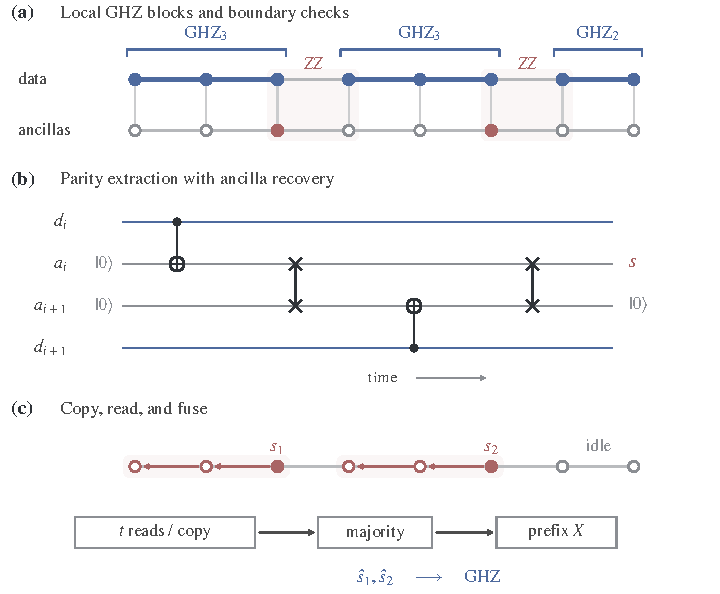
\includegraphics[width=4.8in]{FigS2.pdf}
\caption{\textbf{GHZ preparation with protected boundary parities.}
(a) Two rows support three local GHZ blocks of lengths $3,3,2$.
(b) The four-gate boundary gadget stores the neighboring $ZZ$ parity
in $a_i$ and restores the borrowed qubit $a_{i+1}$ to zero.
(c) Copying each parity through its left block and reading every copy
$t$ times protects the fusion. Majority decoding followed by prefix
$X$ corrections joins the blocks. The short final block needs no
outgoing parity record.}
\label{fig:Sghz}
\end{figure}



\FloatBarrier
\section{Preparing metrological resources}
\label{sm:qfi}

Place one sensor in each of $N$ consecutive cells and encode the phase
after preparation by $e^{-i\theta G}$, with $G=\sum_i g_i$,
$g_i=g_i^\dagger$, and $\|g_i\|\le1/2$. The generator acts only on the
sensors, but the final measurement can also use the preparation record
$\boldsymbol Y$ and all ancillas. Separable probes have $\FQ\le N$,
whereas GHZ reaches $N^2$ for $G=\tfrac12\sum_i Z_i$~\cite{TothApellaniz2014}.
Here noise acts during preparation. For noise acting on an already
prepared probe, see Refs.~\cite{Lopez2019,Len2022,Zhou2023}.

For interaction depth $d$ and at most $R$ reports per cell, set
$s=2d+2$ and $\alpha=(2p)^{Rs}$. The prepared state satisfies
\begin{align}
 \FQ(\rho_{\mathrm{out},\boldsymbol Y},G)
 &\le N+2\sum_{r=1}^{N-1}(N-r)
       (1-\alpha)^{\lfloor(r-1)/s\rfloor}
 \nonumber\\
 &\le \min\left\{N^2,\,
       N\left(1+\frac{2s}{\alpha}\right)\right\}.
 \label{eq:qfi-finite}
\end{align}
Here $\rho_{\mathrm{out},\boldsymbol Y}$ includes any retained preparation ancillas.
For each individual reported record $\boldsymbol y$ of nonzero probability, the
same inequalities hold with $\alpha$ replaced by
$\widehat\alpha=[p/(1-p)]^{Rs}$. They consequently hold after arbitrary
classical selection of preparation records, at any positive yield. This
selection does not include an additional, unrestricted quantum filter on
the entire sensor array.
Neither bound assumes uniformly distributed outcomes or a specified
correction code.

To prove the bound, resolve the artificial replacement flags, their
independent report values, and controller randomness into a variable $z$.
For fixed $z,\boldsymbol y$, let $\rho_{z,\boldsymbol y}$ denote the normalized prepared state,
averaged over the unobserved true outcomes. Since preparation precedes
encoding, the weights $p(z,\boldsymbol y)$ do not depend on $\theta$. Convexity of
quantum Fisher information and its variance bound imply
\begin{equation}
 \FQ(\rho_{\mathrm{out},\boldsymbol Y},G)
 \le\sum_{z,\boldsymbol y}p(z,\boldsymbol y)\FQ(\rho_{z,\boldsymbol y},G)
 \le4\sum_{z,\boldsymbol y}p(z,\boldsymbol y)
          \operatorname{Var}_{\rho_{z,\boldsymbol y}}(G).
 \label{eq:qfi-conditional-variance}
\end{equation}
For sensors $i,j$ separated by $r$ cells, choose
$\lfloor(r-1)/s\rfloor$ disjoint windows strictly between them.
If any window contains only replacement reports, the fixed-record
cut-deletion argument makes their two-sensor marginal a product.
Their conditional covariance therefore vanishes. Otherwise its absolute
value, for the observables $g_i$ and $g_j$, is at most $1/4$.
The probability of having no such window is
$(1-\alpha)^{\lfloor(r-1)/s\rfloor}$.
Summing these covariance bounds and using
$\operatorname{Var}(g_i)\le1/4$ gives the first inequality in
Eq.~\eqref{eq:qfi-finite}. The geometric sum over all positive separations
is $s/\alpha$, giving the second inequality. The argument also covers retained ancillas because the variance of $G$
depends only on one- and two-sensor marginals.

For a specified $\boldsymbol y$, resolve only $z$ and use the record-wise CP-order
bound. Taking its trace on the preparation input bounds the conditional
probability of having no replacement-only window by
$(1-\widehat\alpha)^{\lfloor(r-1)/s\rfloor}$.
The same covariance argument proves the individual-record statement.
Convexity then covers any classical selection and mixture of records.
Using the unconditioned variance would count correlations created by
classical feedback. An equal mixture of $\ket{0^N}$ and $\ket{1^N}$
has quadratic variance for $G=\frac12\sum_i Z_i$ but zero quantum
Fisher information for the same generator.

For duration $D$, the bounds $R\le bD$ and $d\le D$ yield, at fixed $p,b$,
\begin{equation}
 \FQ\le\min\{N^2,\,
 C N(D+1)\exp[c_{p,b}D(D+1)]\}.
 \label{eq:qfi-duration}
\end{equation}
The constants can also be chosen for the individual-record bound.
More generally, $\FQ\ge c_0N^{1+\gamma}$ with fixed $c_0,\gamma>0$
requires $D=\Omega(\sqrt{\gamma\ln N})$, by taking logarithms
in Eq.~\eqref{eq:qfi-duration}.
Consequently, preparing any state with $\FQ\ge\eta N^2$, for fixed
$0<\eta<1$, requires $D=\Omega(\sqrt{\ln N})$.
With one terminal readout round, $R=O(1)$ instead gives
$D=\Omega(\ln N)$.

For $G=\frac12\sum_i Z_i$, the GHZ block-fusion construction attains both scalings. Let block $a$
contain $n_a$ sensors, and let every decoded boundary parity have
independent error probability $q$. Its output is a mixture of positive-phase
GHZ domain states, with each domain constant inside a block. Every component
has $X^{\otimes N}=+1$, whereas $G$ maps this subspace to the orthogonal
$-1$ subspace. The spectral formula for quantum Fisher information thus
reduces to $\FQ=4\tr(\rho G^2)$. Independent boundary errors give
\begin{align}
 \FQ
 &=\sum_{a,b}n_an_b(1-2q)^{|a-b|}
 \nonumber\\
 &=\ell^2\left[M+2\sum_{r=1}^{M-1}(M-r)(1-2q)^r\right]
 \quad (n_a=\ell).
 \label{eq:qfi-exact}
\end{align}
In particular, $\FQ\ge N^2(1-2q)^{M-1}$.
Spatial copies and repeated readout give
$q\le e^{-\kappa_p\ell t}$ in duration $O(\ell+t)$.
Choosing $\ell,t$ proportional to $\sqrt{\ln N}$ with sufficiently
large coefficients gives any fixed fraction of $N^2$. A single
readout round achieves the same fraction with $\ell=O(\ln N)$.
For equal blocks ($N=\ell M$), summing the geometric series in
Eq.~\eqref{eq:qfi-exact} gives $\FQ/(N\ell)\to(1-q)/q$ as
$M\to\infty$, even while the fidelity to a single GHZ state falls
as $(1-q)^{M-1}$.

\FloatBarrier
\section{Detector likelihoods and rare postselection}
\label{sm:detector}

Suppose a true binary outcome $u$ is reported through a fresh use of a
detector $W(\cdot|u)$, independently of the past given $u$. Write $w_0,w_1$
for the two report densities with respect to the sum $\nu$ of the two laws. Define
\begin{equation}
 \kappa_W=-\ln\int\sqrt{w_0w_1}\,d\nu,\qquad
 \Lambda_W=\operatorname*{ess\,sup}_{y}
 \left|\ln\frac{w_0(y)}{w_1(y)}\right|.
 \label{eq:detector-likelihoods}
\end{equation}
If an event has positive probability for just one input, then $\Lambda_W=\infty$.
For a finite alphabet the integral reduces to the usual sum of square roots
of probability products. The Bhattacharyya distance $\kappa_W$ measures
distinguishability under repeated readout. The largest log-likelihood
ratio $\Lambda_W$ measures how decisive one report can be. It is the
larger of the two directional max-divergences, the Thompson distance
appearing in postselected hypothesis testing~\cite{Regula2024}.
For symmetric binary flips the two quantities reduce to $\kappa_p$ and
$\Lambda_p$. Related questions concern detector simulation with unrestricted
resources~\cite{Byrne2026} and communication through a prescribed
postselected channel~\cite{Ji2024}.

The two inputs share a report component of density $\min(w_0,w_1)$.
Its weight $\eta_W=\int\min(w_0,w_1)\,d\nu$ is one minus their total
variation distance. The averaged-channel bound uses $\eta_W$ in place of
the binary replacement probability $2p$.

For an instrument $\{\mathcal M_0,\mathcal M_1\}$, report $y$ induces the
map $\mathcal A_y=\sum_u w_u(y)\mathcal M_u$. Its input-independent
contribution $(\min_u w_u(y))(\mathcal M_0+\mathcal M_1)$ dominates
$e^{-\Lambda_W}\mathcal A_y$ in CP order because
$\min_v w_v(y)\ge e^{-\Lambda_W}w_u(y)$ for both true values.
Integration gives $\eta_W\ge e^{-\Lambda_W}$ for unused slots.
Equations~\eqref{eq:branch-domination} and~\eqref{eq:uniform-herald}
and the product contribution in Theorem~\ref{thm:range} therefore obey
the same bounds with $\Lambda_W$ in place of $\Lambda_p$ whenever
$\Lambda_W<\infty$. For continuous outputs the comparison holds almost
everywhere and after selection of any positive-probability set of records.

Independence cannot be replaced by finite-range correlations and full
support. For one type of Bell report, let the error at interface $i$ be
$E_i=B_i\oplus B_{i+1}$, with independent
$B_i\sim\operatorname{Bernoulli}(\theta)$ and $0<\theta<1/2$.
Collections separated by more than one interface are independent,
so the stationary noise is one-dependent. Every finite error string has positive
probability, and each report has error $p=2\theta(1-\theta)$.
Nevertheless, its correction-parity error is
$\bigoplus_{i=1}^M E_i=B_1\oplus B_{M+1}$, also of probability $p$,
independently of $M$. Use independent copies of this process for the two
Bell-bit types and for each readout round. Majority decoding of each
\emph{whole correction parity} then reaches any fixed fidelity using a
fixed number of rounds at every distance. Thus finite correlation length
and full support alone do not imply the transmission bound.

Independence is sufficient, not necessary. For example, draw an
input-independent latent variable $\lambda$ once per run. Conditional on
$\lambda$, let all reports have independent binary flips with a rate
$p_\lambda\in[p_{\min},1/2]$, where $p_{\min}>0$ is fixed.
Theorem~\ref{thm:range} holds uniformly in $\lambda$ with
$\Lambda_{p_{\min}}=\ln[(1-p_{\min})/p_{\min}]$. For each actual record, the state is a
mixture of the corresponding separable conditional states, even though
that record updates the distribution of $\lambda$. This proves the same
strict range bound for this class of common-cause correlations. No claim
is made for arbitrary finite-range correlated noise.

\paragraph*{Optimal duration for general detectors.}
Fix the detector, an accuracy $0<\eps<1/2$, and a strip of
fixed width supporting the transmission construction. With ideal quantum
operations, fresh independent reports, and arbitrary positive yield,
Eq.~\eqref{eq:detector-likelihoods} gives
\begin{equation}
 D_{\rm her}^{\star}(L;W)=
 \begin{cases}
  \Theta(L),&\Lambda_W=0,\\
  \Theta_W(\sqrt{\ln L}),&0<\Lambda_W<\infty,\\
  \Theta(1),&\Lambda_W=\infty.
 \end{cases}
 \label{eq:detector-classification}
\end{equation}
For $\Lambda_W=0$, the two report laws coincide. Freezing any record leaves
a local trace-preserving circuit. Transmission then requires linear
depth, which a SWAP circuit attains.

For $\Lambda_W=\infty$, the likelihood ratio is unbounded in at least
one direction. Exchanging the two true values if needed, every finite
$T$ admits a set $A_T$ of positive $\nu$-measure on which
$w_0(y)\ge e^T w_1(y)$.
The constant-depth wire has $k=2L$ independent uniform Bell bits,
independently of any reference input [Eq.~\eqref{eq:wire-kraus}].
Accept when all reports lie in $A_T$ and decode them as zero. Then
\begin{equation}
 \begin{aligned}
 q_T&=\frac{W(A_T|1)}{W(A_T|0)+W(A_T|1)}\le e^{-T},\\
 a_T&=\left[\frac{W(A_T|0)+W(A_T|1)}2\right]^k>0.
 \end{aligned}
 \label{eq:detector-one-tail}
\end{equation}
The yield is input-independent, and the accepted Pauli channel has error at most $ke^{-T}$. Choosing $T=\ln(k/\eps)$ proves achievability.

For $0<\Lambda_W<\infty$, the branchwise converse gives the lower
bound. For any detector, likelihood-ratio decoding of $m$ independent
reports of a uniform bit gives
\begin{equation}
 q_m\le\tfrac12e^{-m\kappa_W}.
 \label{eq:detector-repetition}
\end{equation}
Since $\kappa_W>0$ whenever the laws differ, spatial copies and repeated
readout attain square-root logarithmic duration, also for asymmetric
detectors. The Bhattacharyya distance equals the Chernoff information
for binary symmetric readout. For general report laws the Chernoff information lies between
$\kappa_W$ and $2\kappa_W$.

\paragraph*{Uniform information cost for a general detector.}
The deterministic comparison extends beyond binary symmetric readout.
For $0<\kappa_W<\infty$, choose an input-independent report density
$g(y)=e^{\kappa_W}\sqrt{w_0(y)w_1(y)}$.
For either true value $u$, the integral of $g^2/w_u$ on the common
support is at most $e^{2\kappa_W}$. On complete histories of
true outcomes and reports, changing the reporting kernel in window $j$
multiplies the positive history operator by
$\mathcal L_j=\prod_{i\in j}g(y_i)/w_{u_i}(y_i)$.
Dummy reports drawn from $W(\cdot|0)$ pad unused slots and integrate
out without any physical measurement.

Order the slots chronologically, breaking ties in a fixed order.
Given the prior history and the current true outcome $u$, the next
multiplier $g(Y)/w_u(Y)$ has mean one and second moment at most
$e^{2\kappa_W}$. Write $\mathcal L_j(t)$ for the partial product over
the first $t$ slots and $N_j(t)$ for the number of those slots in window
$j$. A slot updates at most one of two disjoint windows, so
$\mathcal L_j(t)\mathcal L_k(t)$ is a mean-one martingale for $j\ne k$.
The second-moment bound makes $e^{-2\kappa_W N_j(t)}\mathcal L_j(t)^2$
a supermartingale starting at one. With $N_j(t)\le n$ this gives
$\mathbb E\mathcal L_j^2\le e^{2\kappa_W n}$.
The changed channel is entanglement breaking by the window geometry.
Applying the trace-norm mixture estimate to any reference--input state
and taking the supremum gives
\begin{equation}
 \inf_{\mathcal S\in\mathrm{EB}}
 d_\diamond(\channel,\mathcal S)
 \le\frac12\sqrt{\frac{e^{2\kappa_W R(2d+2)}-1}{K}}.
 \label{eq:general-statistical-eb}
\end{equation}
The constants in this bound are independent of the adaptive quantum
outcome probabilities. Combining it with Eq.~\eqref{eq:detector-repetition}
proves the deterministic part of Eq.~\eqref{eq:uniform-information-time}
with $\alpha=\kappa_W$, uniformly over detector laws at fixed accuracy.
At $\kappa_W=0$ the laws coincide and coherent transport is necessary.
At $\kappa_W=\infty$ their supports are disjoint up to null sets, so
constant-depth teleportation suffices.

At nonnegligible yield, the overlap $\eta_W$ suffices. Write
$K=\lfloor(L-1)/(2d+2)\rfloor$. Any receiver-side trace-nonincreasing CP selection with Bell-input
probability $a$ and accepted fidelity at least $1-\eps$ obeys
\begin{equation}
 a(1-2\eps)\le
 \left(1-\eta_W^{R(2d+2)}\right)^K.
 \label{eq:detector-yield-bound}
\end{equation}
Indeed, selection cannot increase the unnormalized weight of the
non-entanglement-breaking contribution, while the remaining contribution
has Bell overlap at most half its trace. This includes receiver quantum
filtering. For fixed $0<\eta_W<1$ and $a\ge a_0L^{-\gamma}$, with fixed
$a_0>0$ and $\gamma\ge0$, the inequality and $d\le D$, $R\le bD$ force
$D=\Omega_W(\sqrt{\ln L})$. Equation~\eqref{eq:detector-repetition}
provides a deterministic matching construction.

\paragraph*{Mean completion time.}
A small success probability also costs time if rejected stages are
included. Fix a detector with distinct but overlapping report laws,
$0<\eta_W<1$, and a target Bell fidelity $1-\eps>1/2$.
Allow the protocol to retain quantum memory across stages and stop at
a record-dependent duration $T$. Suppose it completes almost surely,
its final averaged Bell fidelity is at least $1-\eps$, and
$\overline T=\mathbb E[T]<\infty$, with both expectation and fidelity evaluated
on the Bell input. All quantum operations and raw reports, including
those in rejected stages, are counted. Then
\begin{equation}
 \inf\mathbb E[T]=\Theta_W(\sqrt{\ln L})
 \label{eq:mean-completion-time}
\end{equation}
for fixed accuracy and width supporting the construction.

To prove the lower bound, set $c=2/(1-2\eps)$ and truncate the protocol
at $\lceil c\overline T\rceil$, accepting only completed histories. Markov's
inequality bounds the omitted probability by $1/c$. If $\omega_\le$
is the resulting unnormalized Bell output, then
\begin{equation}
 2\tr(\Phi^+\omega_\le)-\tr\omega_\le
 \ge 1-2\eps-\frac1c=\frac{1-2\eps}{2}.
 \label{eq:mean-truncation}
\end{equation}
Indeed, removing a set of probability $\delta$ can reduce this linear
Bell advantage by at most $\delta$. For the truncated protocol, the
unconditional decomposition bounds this accepted advantage by the
non-entanglement-breaking weight
$\Pi_{\rm av}=(1-\eta_W^{R(2d+2)})^K$. Selection cannot increase that weight, so
$\Pi_{\rm av}\ge2\tr(\Phi^+\omega_\le)-\tr\omega_\le\ge(1-2\eps)/2$.
Using $d\le\lceil c\overline T\rceil$ and
$R\le b\lceil c\overline T\rceil$ now proves
$\overline T=\Omega_W(\sqrt{\ln L})$. The deterministic construction based on
Eq.~\eqref{eq:detector-repetition} attains the upper bound. The lower bound uses a fixed Bell-fidelity advantage on the Bell
input, so it also applies to worst-case expected duration.

The readout dependence of this mean-time law is also uniform.
For the truncated protocol, an entanglement-breaking comparison channel
has nonpositive accepted Bell advantage. Equation~\eqref{eq:general-statistical-eb}
therefore implies
$(1-2\eps)/2\le\sqrt{[e^{2\kappa_W n}-1]/K}$.
The lower-bound argument of Eq.~\eqref{eq:uniform-information-time}
applies with $\alpha=\kappa_W$, and the deterministic wire attains it.
For $x_\alpha=O(1)$, the bound $\mathbb E[T]\ge1-2\eps$ from separability
of zero-layer outputs absorbs the truncation ceiling.
Charging failed
stages restores the reliable-transmission information cost even when
arbitrarily rare fixed-duration selection is possible.

Full support alone does not imply the arbitrary-yield, fixed-duration
bound for an unbounded analog record. Consider the idealized detector
\begin{equation}
 Y=(-1)^u\mu+\sigma Z,\qquad Z\sim\mathcal N(0,1),
 \qquad \mu,\sigma>0 .
 \label{eq:analog-detector}
\end{equation}
Here $\kappa_W=\mu^2/(2\sigma^2)$ and $\eta_W=2\Phi(-\mu/\sigma)>0$,
where $\Phi$ is the standard normal cumulative distribution function.
The log-likelihood ratio grows linearly with $Y$, giving $\Lambda_W=\infty$. Use the constant-depth
neighboring-link teleportation circuit, whose $k=2L$ Bell bits are
independent and uniform, independently of the input state. Decode each
bit by the sign of its analog report and accept only when all reports
satisfy $|Y|\ge y_{\mathrm c}$. For an accepted report, the posterior error is
$[1+\exp(2\mu|Y|/\sigma^2)]^{-1}\le
\exp(-2\mu y_{\mathrm c}/\sigma^2)$. Thus the accepted transmission has
$1-\Fe^{\rm acc}\le k\exp(-2\mu y_{\mathrm c}/\sigma^2)$. Choosing
$y_{\mathrm c}=(\sigma^2/2\mu)\ln(k/\eps)$ gives error at most $\eps$, with
\begin{equation}
 a=\left[\Prb\{|\mu+\sigma Z|\ge y_{\mathrm c}\}\right]^k>0,
 \qquad
 \ln a=-\Theta_{\mu,\sigma}\!\left(
 k[\ln(k/\eps)]^2\right)
 \label{eq:analog-yield}
\end{equation}
in the large-threshold regime. The yield is independent of the unknown
input, so this defines an accepted transmission channel, not merely
successful filtering for a selected input ensemble.

This example assigns no extra cost to retaining arbitrarily large analog
values and relies on their ideal Gaussian tails. The extremely small yield is consistent with
the unconditional bound. Any fixed finite digitizer whose bins have
positive probability for both inputs gives $\Lambda_W<\infty$ and restores
the arbitrary-yield bound. Retaining only the sign reduces the detector
to binary symmetric readout.

\FloatBarrier
\section{Complementary-basis tests}
\paragraph*{Parity measurement.}
For an arbitrary instrument the corrected Bell test gives the one-sided
bound in Eq.~\eqref{eq:bell-bridge-main}. For the circuit of
Fig.~\ref{fig:finite}(b) one can also recover the operation error
from two local measurement settings. Prepare $\ket{++}$ and record the
returned parity. Measure both data qubits in $Z$ on one set of runs
and in $X$ on another. For odd reported parity the local correction
reverses the sign assigned to $Z_B$ and leaves $X_B$ unchanged.
The two residual errors are independent in this circuit, and
Eq.~\eqref{eq:parity-phase-main} gives
\begin{equation}
 1-\eps_{\rm op}=
 \frac{1+\langle Z_A Z_B\rangle_{\rm corr}}{2}\,
 \frac{1+\langle X_A X_B\rangle_{\rm corr}}{2}.
 \label{eq:two-settings-parity}
\end{equation}
Each factor is the probability that the corresponding correction is
right. Extra flips can be introduced in the stored reports before
decoding to change the readout noise independently of the gates.

\paragraph*{Transmission.}
Let $\omega_{QB}=(\id_Q\otimes\channel)(\Phi^+_{QA})$ be the normalized Choi state of the unconditioned transmission channel. Define
\begin{equation}
 P_Z=\frac{\Id+Z_QZ_B}{2},\qquad
 P_X=\frac{\Id+X_QX_B}{2}.
\end{equation}
These commuting projectors obey $P_ZP_X=\Phi^+_{QB}$ and
$P_Z+P_X-\Id\le\Phi^+_{QB}$.
Prepare each of $\ket0,\ket1,\ket+,\ket-$ at the input and measure the
output in its matching basis. Let $\mathcal F_Z,\mathcal F_X$ be the mean correct-label
probabilities within the two bases. Since these input states are real, the Choi identity gives
$\tr(P_Z\omega)=\mathcal F_Z$ and $\tr(P_X\omega)=\mathcal F_X$. Consequently
$\Fe\ge \mathcal F_Z+\mathcal F_X-1$~\cite{Hofmann2005}, and Eq.~\eqref{eq:unconditional}
implies
\begin{equation}
 \mathcal S:=\frac{\mathcal F_Z+\mathcal F_X}{2}\le\frac34+\frac{\Pi_{\rm av}}4 .
 \label{eq:test}
\end{equation}
A channel that measures and prepares in the $Z$ basis has $\mathcal F_Z=1$,
$\mathcal F_X=1/2$, and saturates the classical score $3/4$. The controller must
receive neither the preparation basis nor the input label.
Input preparation and final detector errors must be calibrated separately
from internal reporting errors.
The same witness applies to accepted transmission with input-independent
acceptance probability, using $\Pi$ in place of $\Pi_{\rm av}$.
For input-dependent acceptance the Choi test requires weighting the
basis scores by their acceptance probabilities.



\end{document}
